\clearpage
% \setcounter{page}{1}
\maketitlesupplementary

\section{More Details of LongVALE Benchmark}
\subsection{Quantitative Analysis of Event Boundaries}
\label{sec:boundary}
To quantitatively verify the semantic coherence of segmented events of different modalities, we introduce Max Running Semantic Difference (MRSD), inspired by~\cite{chen2024panda}. For a $n$-second event clip, we compute the embedding for each second as $\{f_{1}, \dots, f_{n}\}$, and get the most significant semantic change within the clip, denoted as:   
\begin{equation}
    \mathrm{max}(\{\mathrm{Diff}(f_{i},f_{i+1}) | i \in [1, n-1]\}).
\end{equation}
We apply ImageBind~\cite{girdhar2023imagebind} and CLAP~\cite{wu2023large} to extract embeddings for visual and audio clips, respectively. 
As in Tab.~\ref{tab:boundary}, for single-modal events, the clips after the second stitching stage effectively avoid being overly fragmentary while maintaining strong semantic coherence.
Further, although semantic shifts may occur between single-modal events within an omni-modal event, no event is truncated, ensuring the semantic integrity of all events from various modalities.


\begin{table}[ht]
  \centering
  \resizebox{\linewidth}{!}{ 
  \begin{tabular}{lccc}
    \toprule
    Method & MRSD-V$\downarrow$ & MRSD-A$\downarrow$ & Avg.len  \\
    \midrule
    Visual event boundary (splitting) & 0.531 & - & 3.0s\\
    Visual event boundary (stitching) & 0.532 & - & 10.7s \\
    \midrule
    Audio event boundary (splitting) & - & 0.676 & 1.5s\\
    Audio event boundary (stitching) & - & 0.703 & 5.8s \\
    \midrule
    Omni-modal event boundary & 0.601 & 0.784 & 16.7s \\
    \bottomrule
  \end{tabular}}
  \caption{Semantic coherence and event length analysis. We randomly sample 1K long videos in our LongVALE. }
  \label{tab:boundary}
  % \vspace{-5mm}
\end{table}

\subsection{More Statistics}
Based on YouTube metadata, we further analyze the distribution of video categories, as shown in Fig.~\ref{fig:category}. It reflects that our LongVALE covers a wide range of video topics. Besides, since our focus is on long-form videos with rich, event-driven storylines, the diversity of their content cannot be easily summarized by just a few simple categories.
Moreover, as shown in Fig.~\ref{fig:word}, we also illustrate the distribution of the lengths of our omni-modal event captions and visualize their word cloud to highlight the rich omni-modality content within the captions.

\begin{figure}[ht]
  \centering
  \setlength{\abovecaptionskip}{1.0mm}
   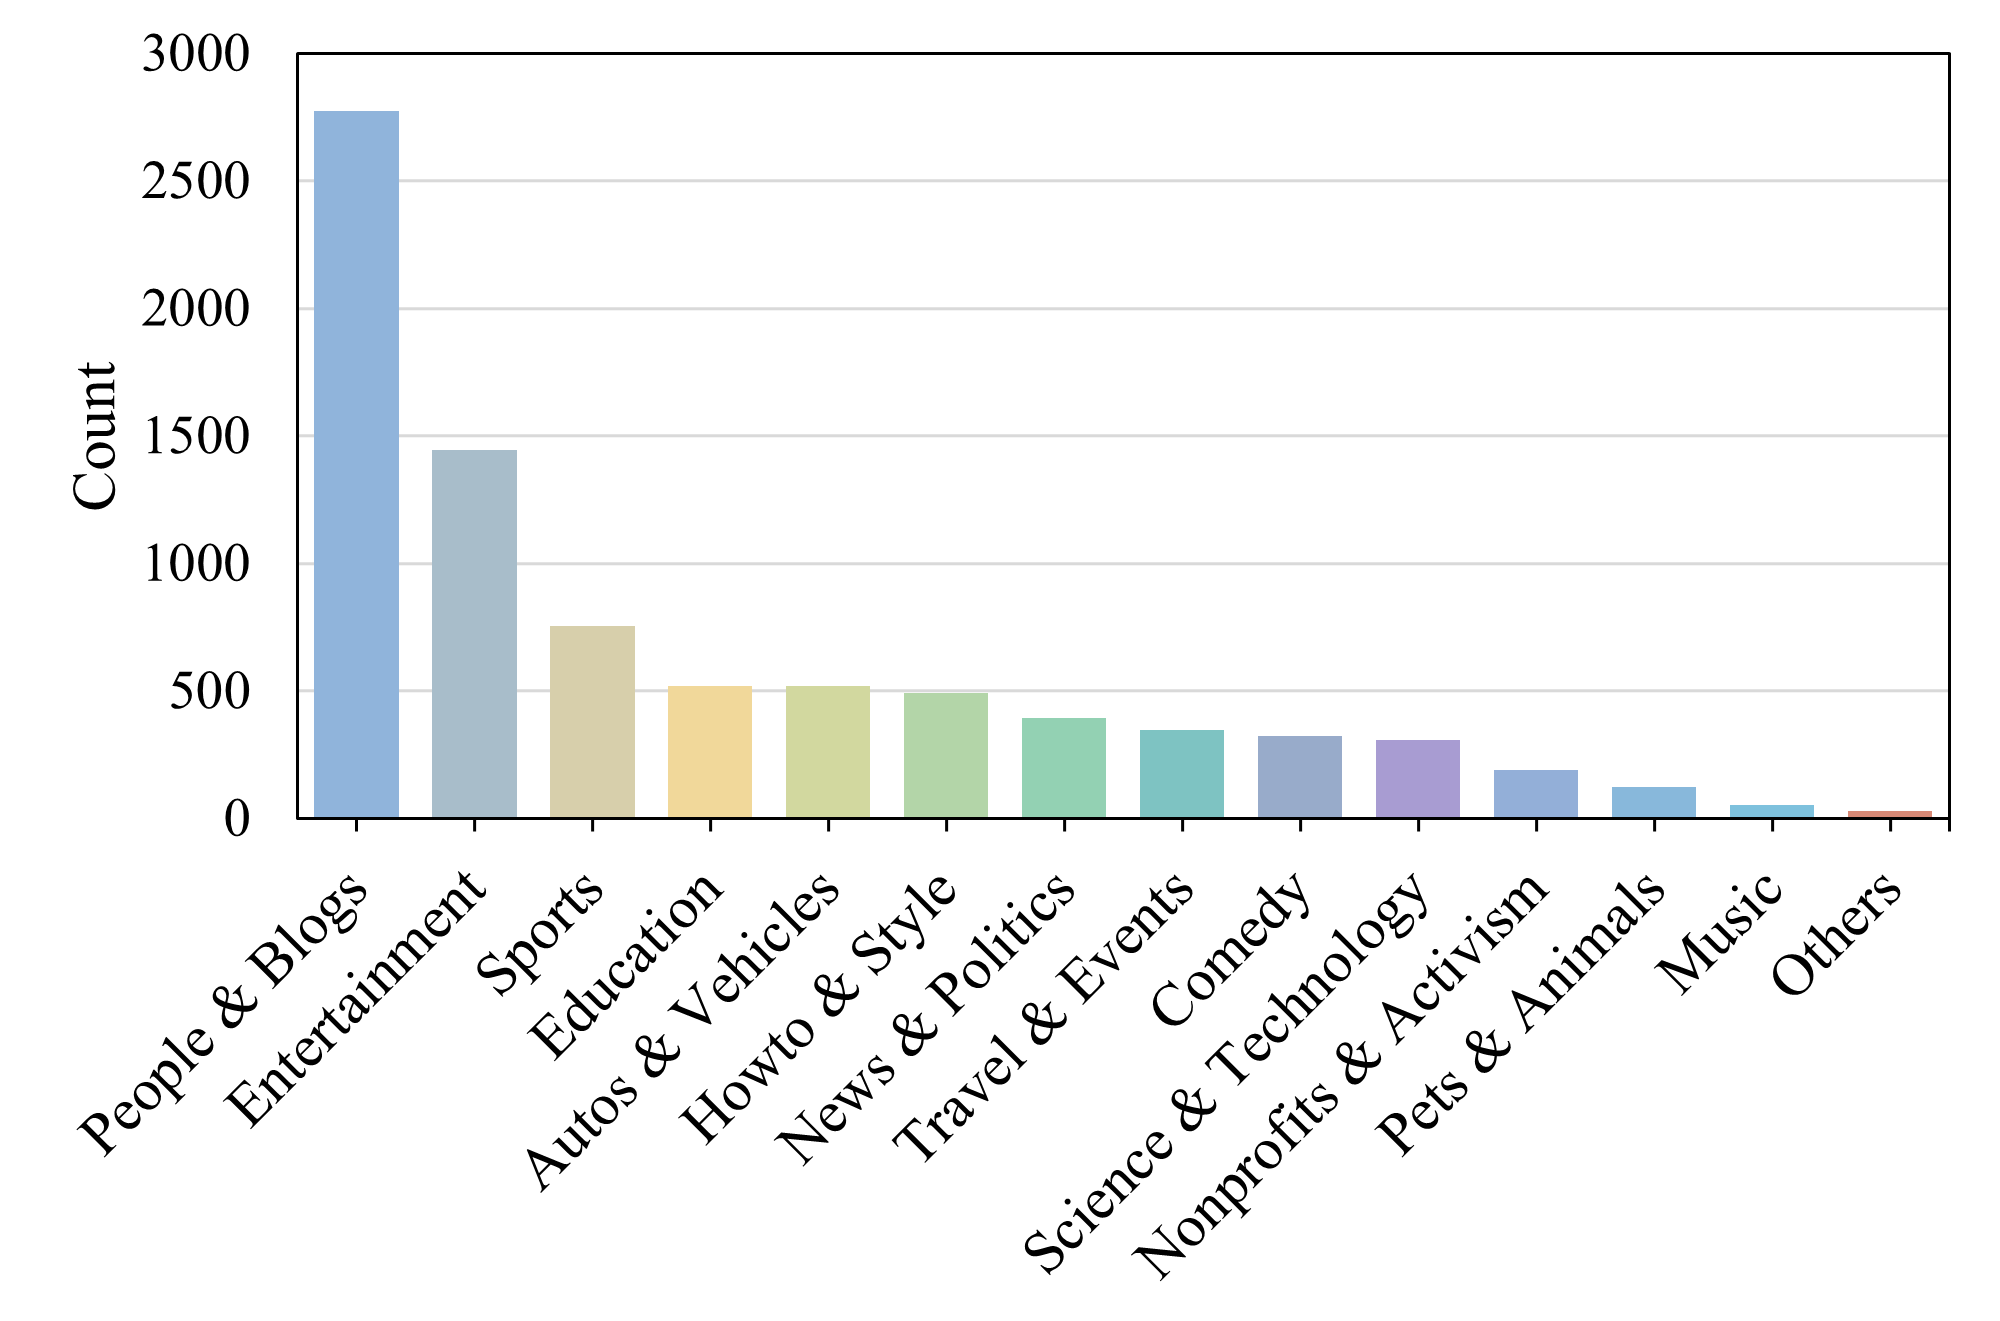
\includegraphics[width=1.0\linewidth]{figures/video_category.png}
   \caption{Distribution of video categories of LongVALE dataset.}
   \label{fig:category}
     \vspace{-4mm}
\end{figure}

\begin{figure*}[ht]
  \centering
  \setlength{\abovecaptionskip}{1.0mm}
   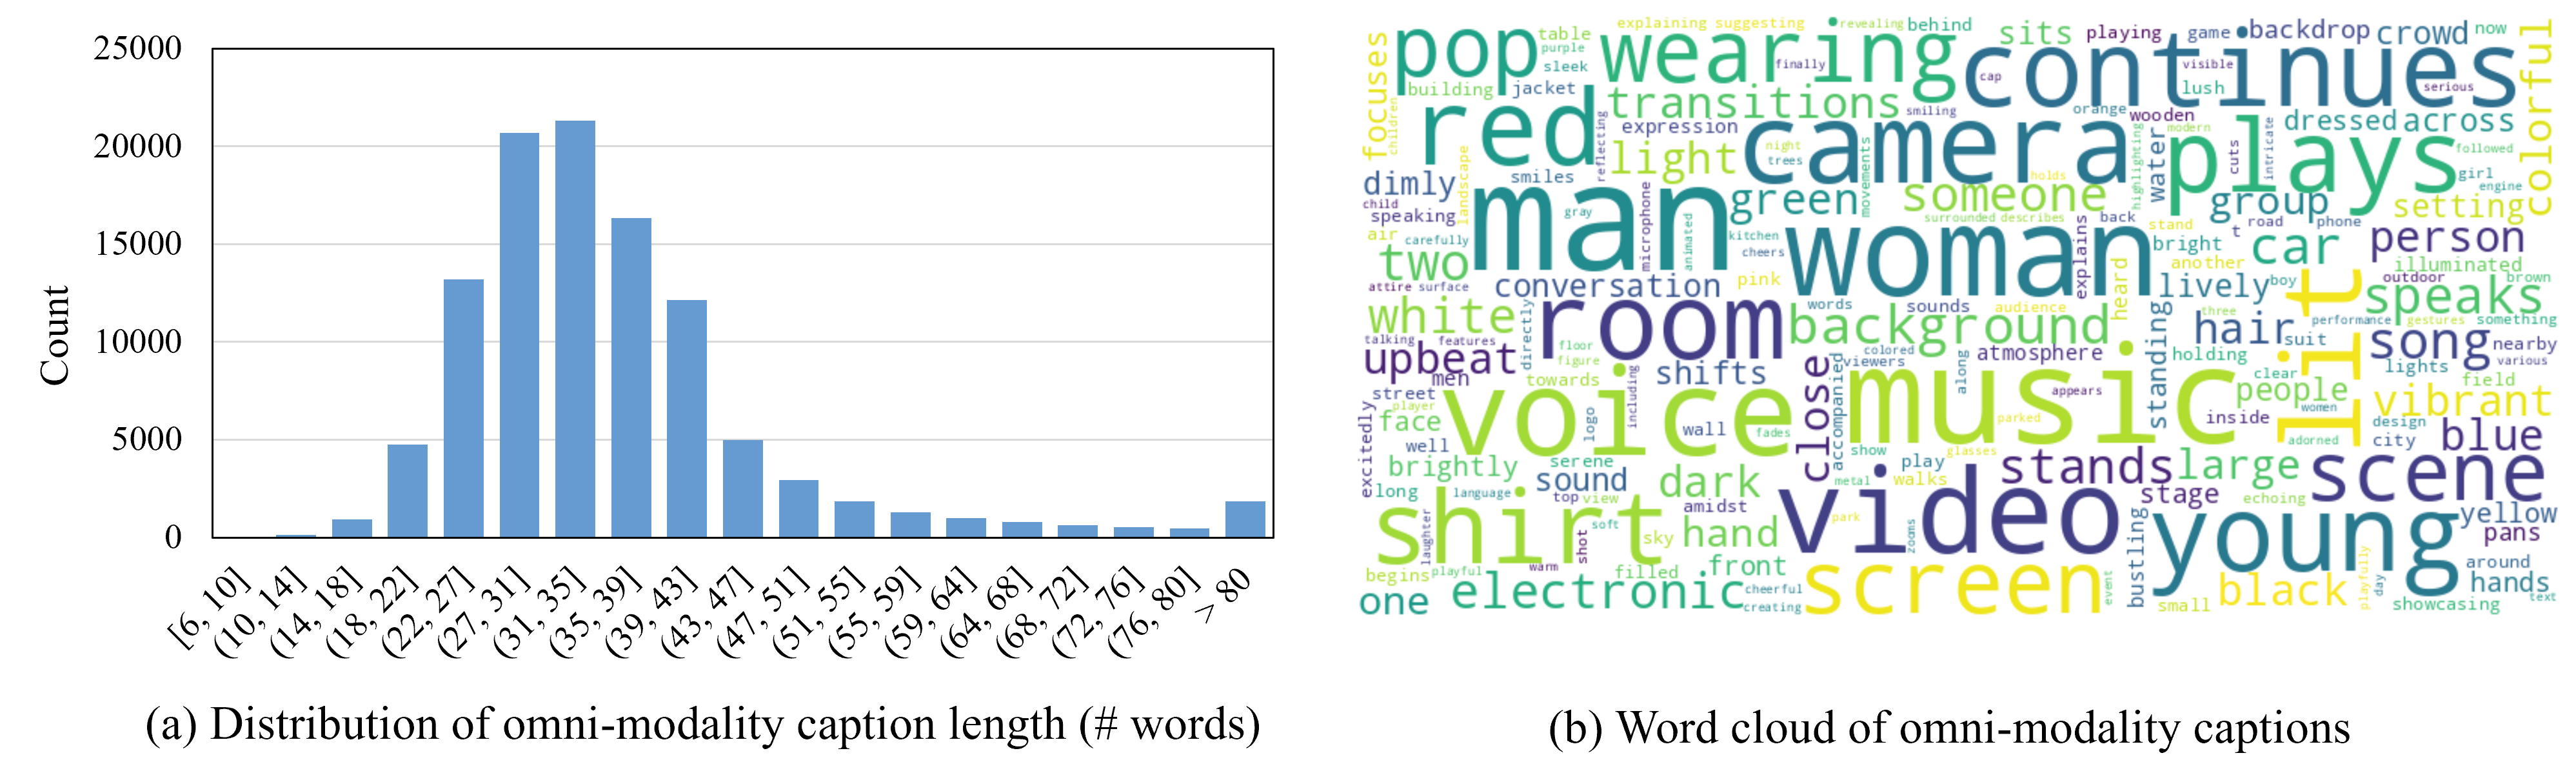
\includegraphics[width=1.0\linewidth]{figures/word_cloud.png}
   \caption{Distribution of omni-modality caption length and word cloud.}
   \label{fig:word}
     \vspace{+4mm}
\end{figure*}

\subsection{Manual Check and Correction}
During the manual check process, annotators are asked to check each omni-modal event and verify whether the caption and the corresponding temporal boundaries are accurate. Besides, videos containing only monotonous background music and speech are filtered out to ensure the dataset includes rich sound types.
Afterward, during the manual correction process, another group of annotators correct all inaccurate annotations and submit the revised versions. 
Totally, we checked 2K videos with each taking 3 minutes, and corrected about 300 errors, totally 115 human hours.
We show the interfaces in Fig.~\ref{fig:manual}

\begin{figure*}[ht]
  \centering
  \setlength{\abovecaptionskip}{1.0mm}
   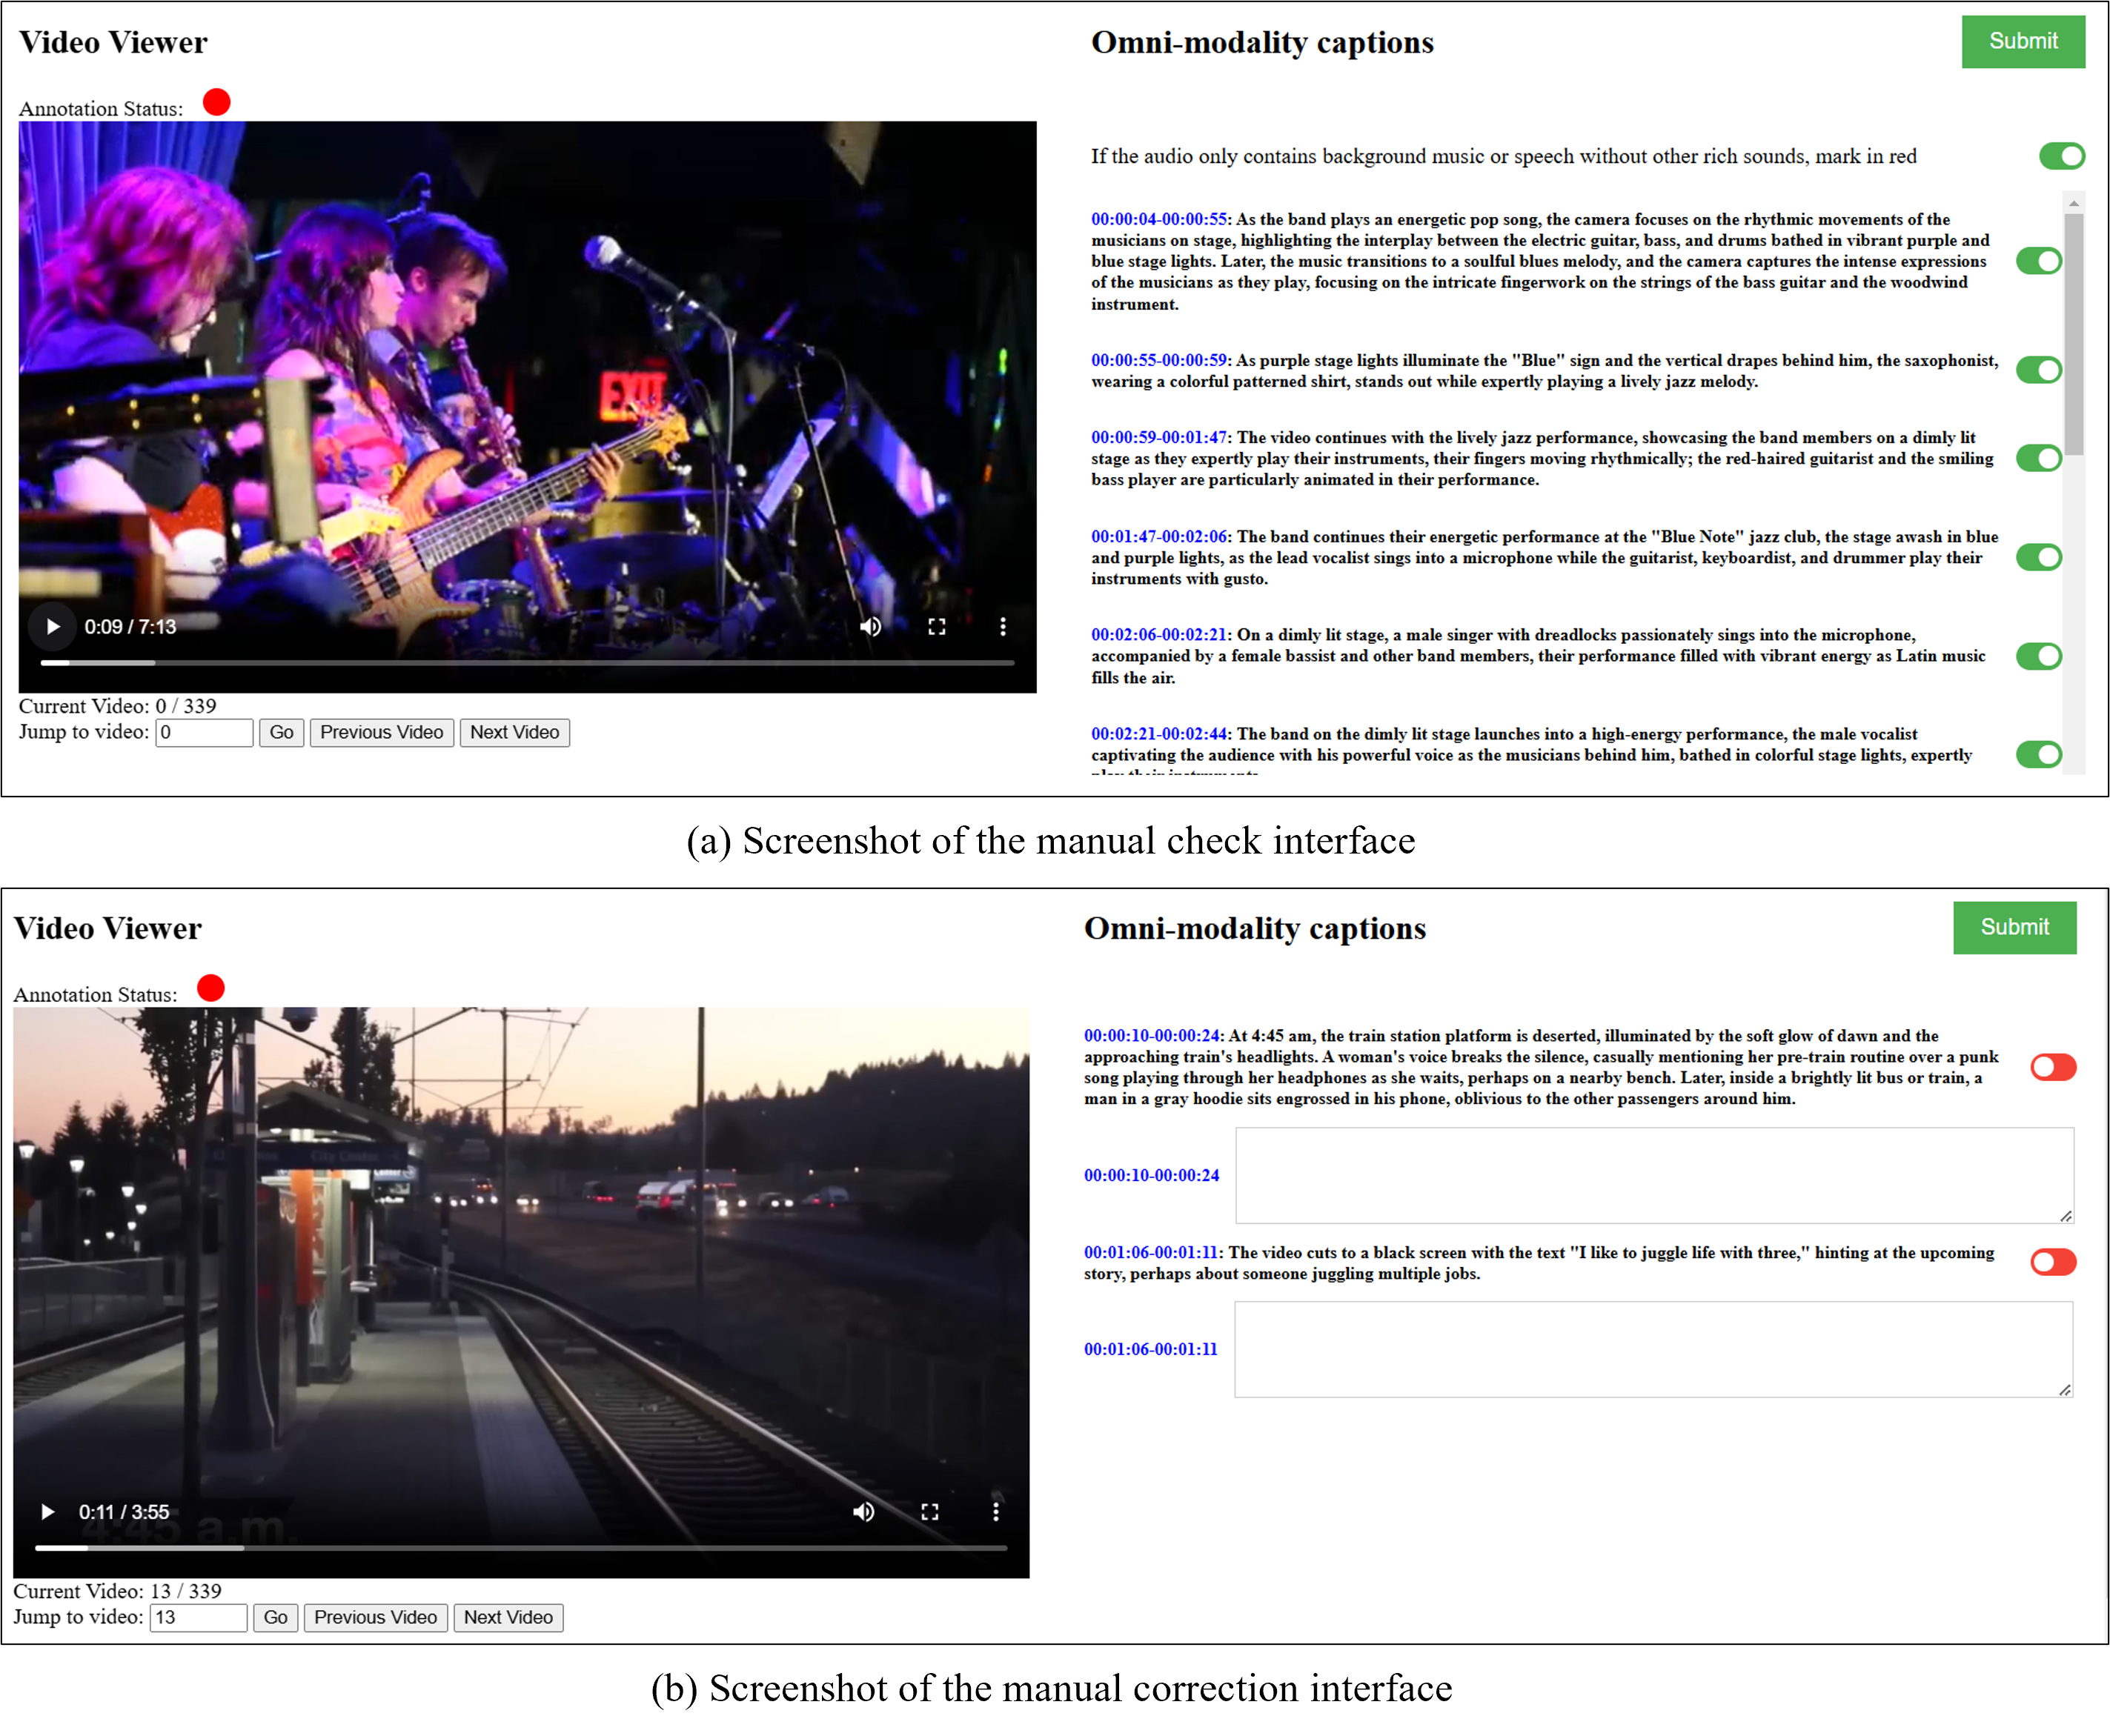
\includegraphics[width=1.0\linewidth]{figures/manual.png}
   \caption{Screenshots of our manual check and correction interfaces.}
   \label{fig:manual}
     % \vspace{+10mm}
\end{figure*}


\subsection{Captioning and AV correlation Prompts}
In Sec.{\color{blue}3.3}, for each segmented video clip, we apply LLaVA-NeXT-Video (34B)~\cite{zhang2024llavanextvideo} to generate a video caption emphasizing dynamic information and apply GPT-4o~\cite{Gpt-4o} to generate keyframe caption emphasizing spatial details. For each segmented audio clip, we apply Qwen-Audio-Chat (7B)~\cite{chu2023qwen} to generate an audio caption, and utilize Whisper-Large-V3~\cite{radford2023robust} to get accurate subtitles. 
Note that we found that the performance of the audio captioner lags significantly behind that of visual models, leading to more hallucination issues, such as generating repetitive sentences or incorrect ASR. To address this, we cleaned up these generations, retaining only general descriptions for each audio event (\eg, "this is a man speaking") while removing the specific speech content. Accurate ASR outputs generated by the advanced speech recognition model~\cite{radford2023robust} were used as replacements.
After obtaining modality-specific captions, we instruct Gemini-1.5-Pro~\cite{Gemini} to integrate and correlate them explicitly. The detailed prompts are shown in Fig.~\ref{fig:video_cap}.
In Sec.{\color{blue}3.5}, we quantitatively identify the characteristics of our omni-modal event captions, including audio-visual correlations and fine-grained temporal dynamics using Gemini-1.5-Pro~\cite{Gemini}. Here, we provide the detailed prompt as shown in Fig~\ref{fig:avc}.


\begin{figure*}[ht]
  \centering
  \setlength{\abovecaptionskip}{1.0mm}
   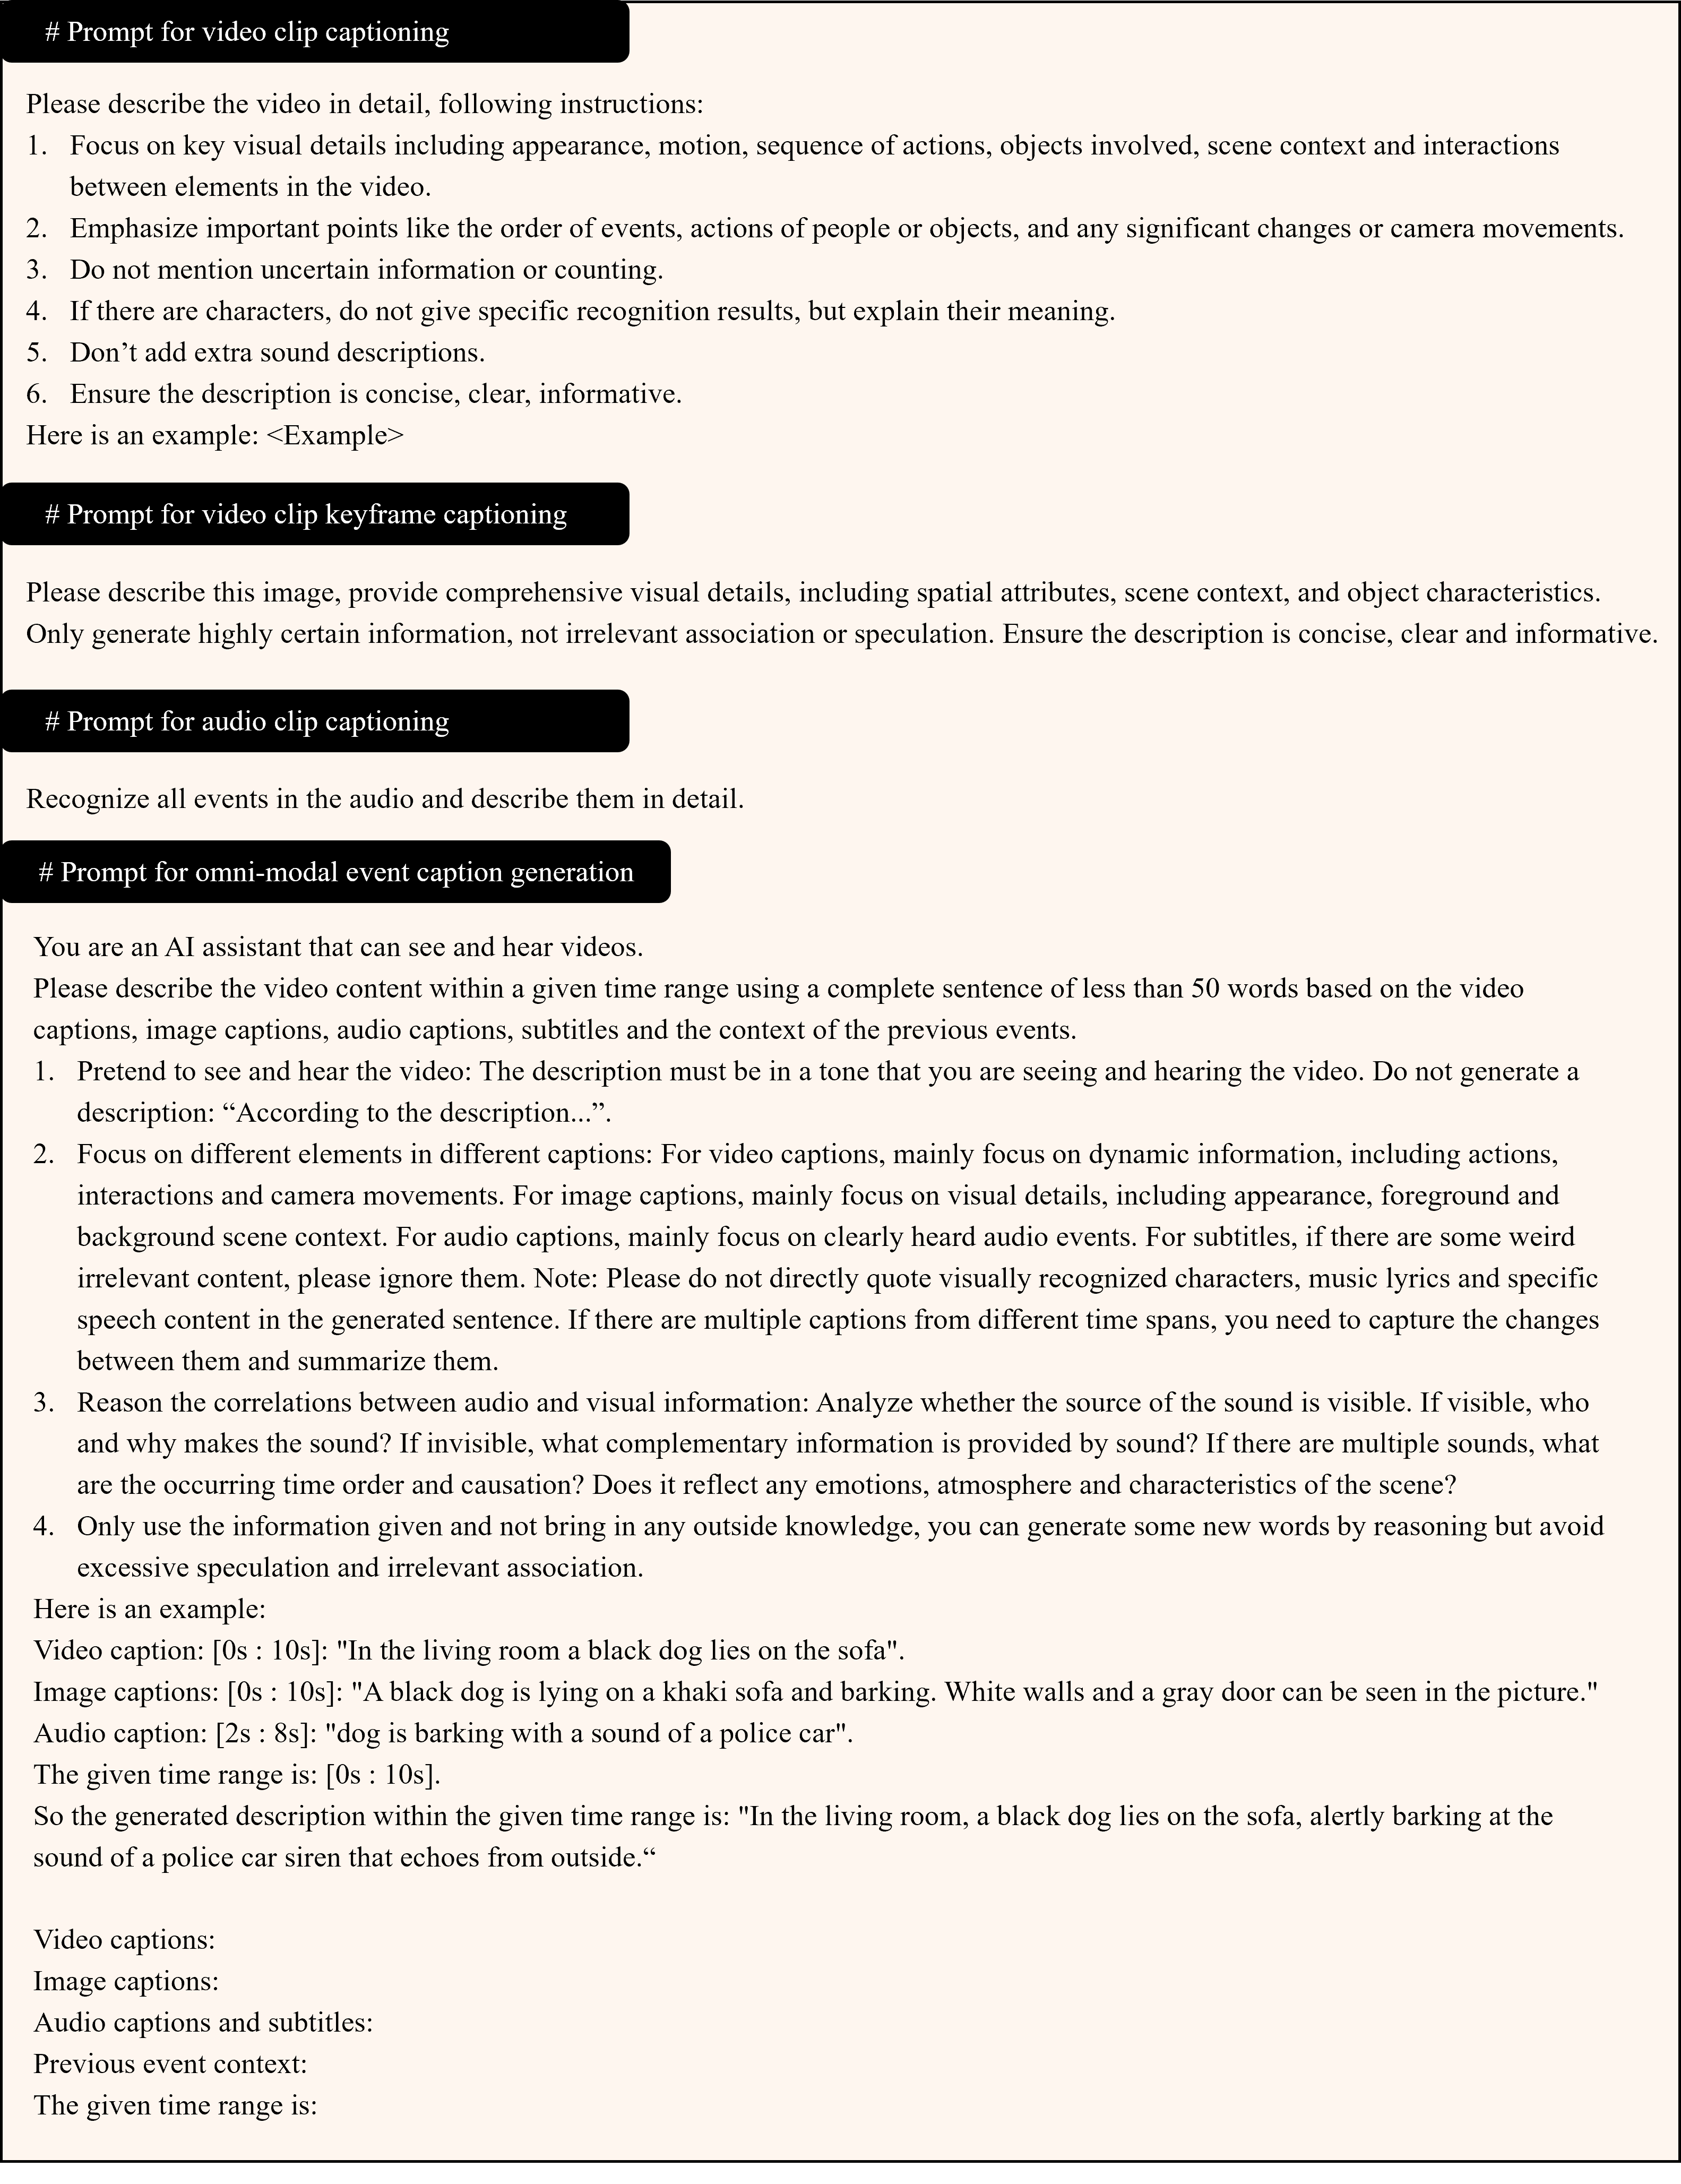
\includegraphics[width=1.0\linewidth]{figures/caption_prompt.png}
   \caption{The prompts for the captioning of video clips, keyframes and audio clips, and integrating them for omni-modal events captions.}
   \label{fig:video_cap}
     % \vspace{-4mm}
\end{figure*}

\begin{figure*}[h]
  \centering
  \setlength{\abovecaptionskip}{1.0mm}
   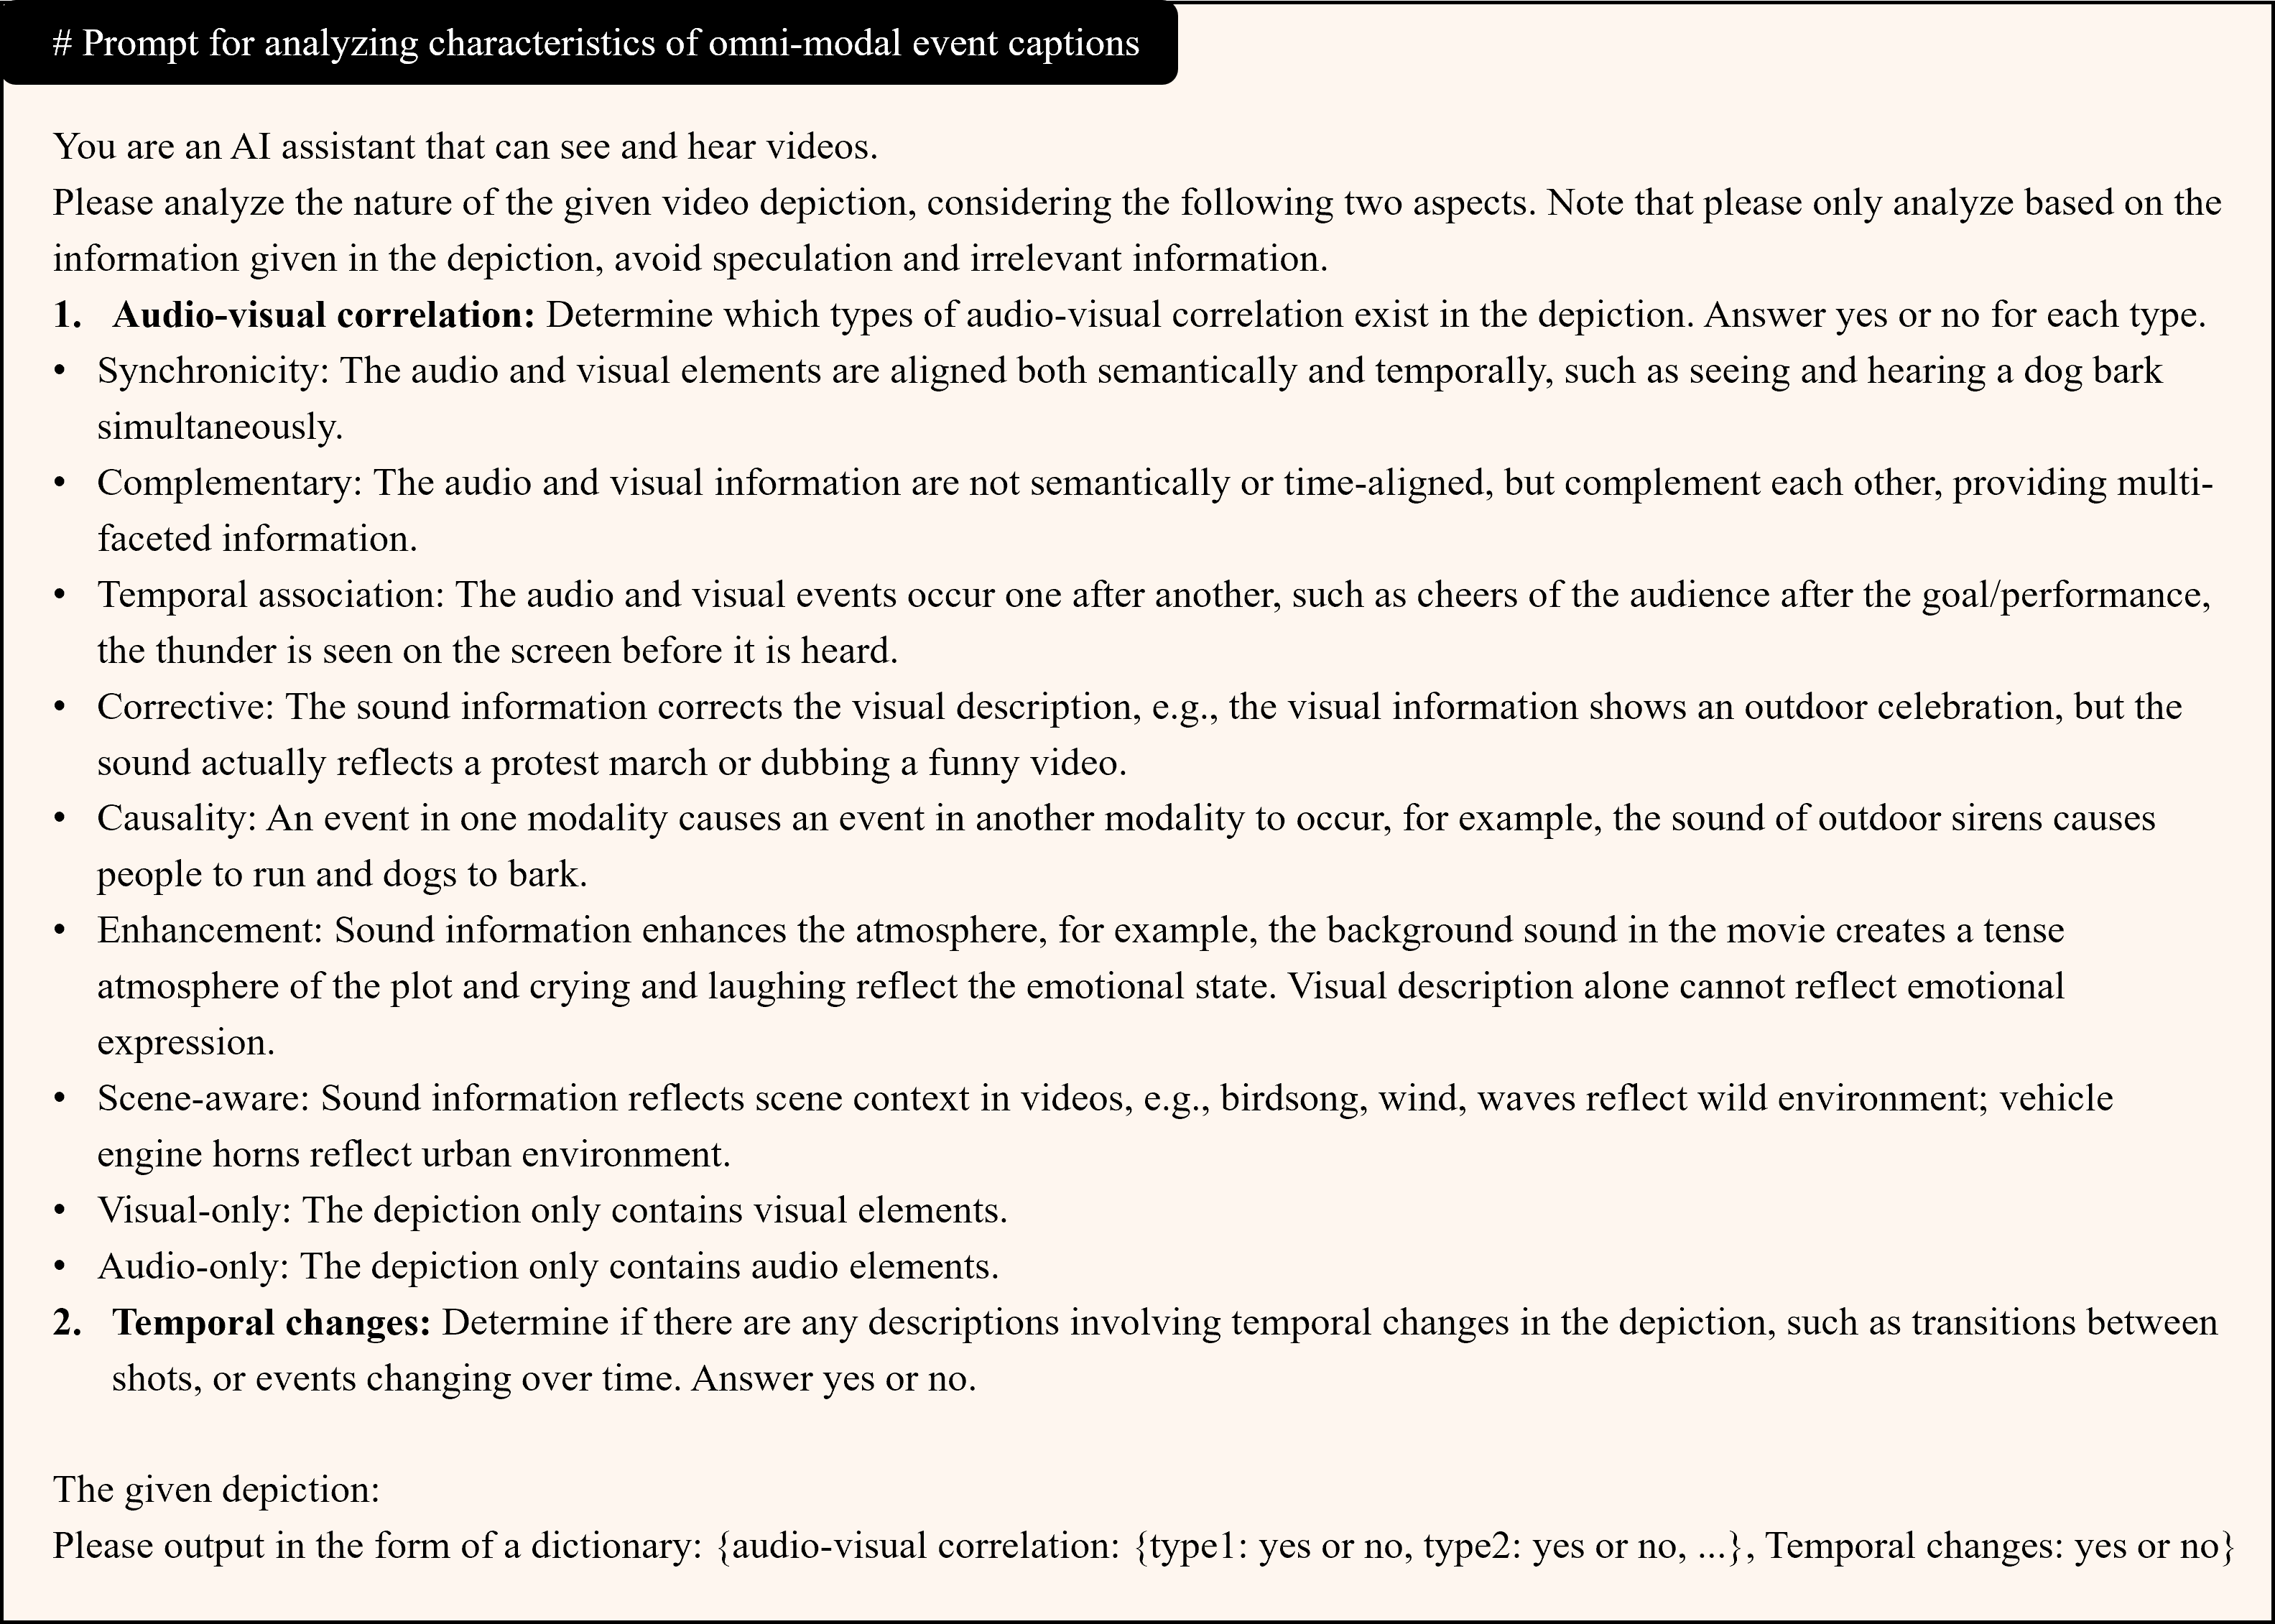
\includegraphics[width=1.0\linewidth]{figures/avc.png}
   \caption{The prompt used to analyze and identify audio-visual correlations and temporal dynamics in our omni-modal event captions.}
   \label{fig:avc}
     % \vspace{-4mm}
\end{figure*}


\section{Task, Model and Training Data Details}
\subsection{Detailed Task Definition}
We extend three fine-grained video tasks to the novel omni-modality domain towards omni-perception of long videos.
These tasks emphasize cross-modal reasoning and fine-grained temporal understanding at the same time. Here, we provide detailed definitions for these tasks.

\noindent\textbf{Omni-modal temporal video grounding.} Given a textual query describing a specific omni-modal event, the model is required to identify the start and end timestamps of the corresponding video segment.

\noindent\textbf{Omni-modal dense video captioning.} The task is more intricate, requiring the model to perform both temporal localization and captioning for all omni-modal events occurring in a given untrimmed video.

\noindent\textbf{Omni-modal segment captioning.} Given a temporal boundary, the task demands the model to generate a caption summarizing the content of the corresponding omni-modal event within the untrimmed video.

\subsection{Detailed Model Architecture}
\noindent\textbf{Multimodal encoders.} Given a video, we utilize a frozen CLIP ViT-L/14~\cite{radford2021learning} as the Visual Encoder to extract visual embeddings $F_{V}=\{v_{i}\}^{N_{v}}_{i=1}$, where $N_{v}$ denotes the number of input video frames. 
Since both non-speech audio (\ie, natural sound and music) and speech provide crucial information for multi-modal video understanding, we employ BEATs~\cite{chen2022beats} and Whisper~\cite{radford2023robust} to extract non-speech audio embeddings $F_{A}=\{a_{i}\}_{i=1}^{N_{a}}$ and speech embeddings $F_{S}=\{s_{i}\}_{i=1}^{N_{s}}$, where $N_{a}$ and $N_{s}$ represent the number of audio and speech embeddings, respectively.
Therefore, the resulting auditory features of these two encoders are complementary and suitable for general audio input.

\noindent\textbf{Multimodal adapters.} We apply linear layers to project the obtained embeddings from different modalities to get visual tokens $\hat{F_{V}}=\{\hat{v_{i}}\}^{N_{v}}_{i=1}$, audio tokens $\hat{F_{A}}=\{\hat{a_{i}}\}_{i=1}^{N_{a}}$, and speech tokens $\hat{F_{S}}=\{\hat{s_{i}}\}_{i=1}^{N_{s}}$ that are aligned with LLM's token space. Subsequently, the obtained token sequences are simply concatenated as:
\begin{equation}
    \mathbf{Z} = \mathrm{Concat}(\hat{F_{V}}, \hat{F_{A}}, \hat{F_{s}}),
\end{equation}
where $\mathbf{Z}\in \mathbb{R}^{N\times d}$, $N=N_{v}+N_{a}+N_{s}$, and $d$ is the hidden dimension of LLM. Note that our model also supports single-modal and dual-modal inputs, allowing for flexible handling of video data with missing modalities.


\noindent\textbf{Large language model.} We use Vicuna-7B-v1.5~\cite{chiang2023vicuna} as our LLM to process concatenated multi-modal tokens $\mathbf{Z}$ and user queries for response generation.

\subsection{Training Data Details}
For boundary perception, we adopted the same template-based data generation strategy as~\cite{huang2024vtimellm} with the same templates, where 20\% of the data is randomly sampled to generate single-turn dialogues (omni-modal dense video captioning), and 80\% is used to generate multi-turn dialogues, \ie, each event is randomly assigned to one of the two tasks (omni-modal temporal video grounding and segment captioning).
For instruction tuning, the prompt used to generate omni-modality dialogues is shown in Fig.~\ref{fig:instruction}.

\begin{figure*}[h]
  \centering
  \setlength{\abovecaptionskip}{1.0mm}
   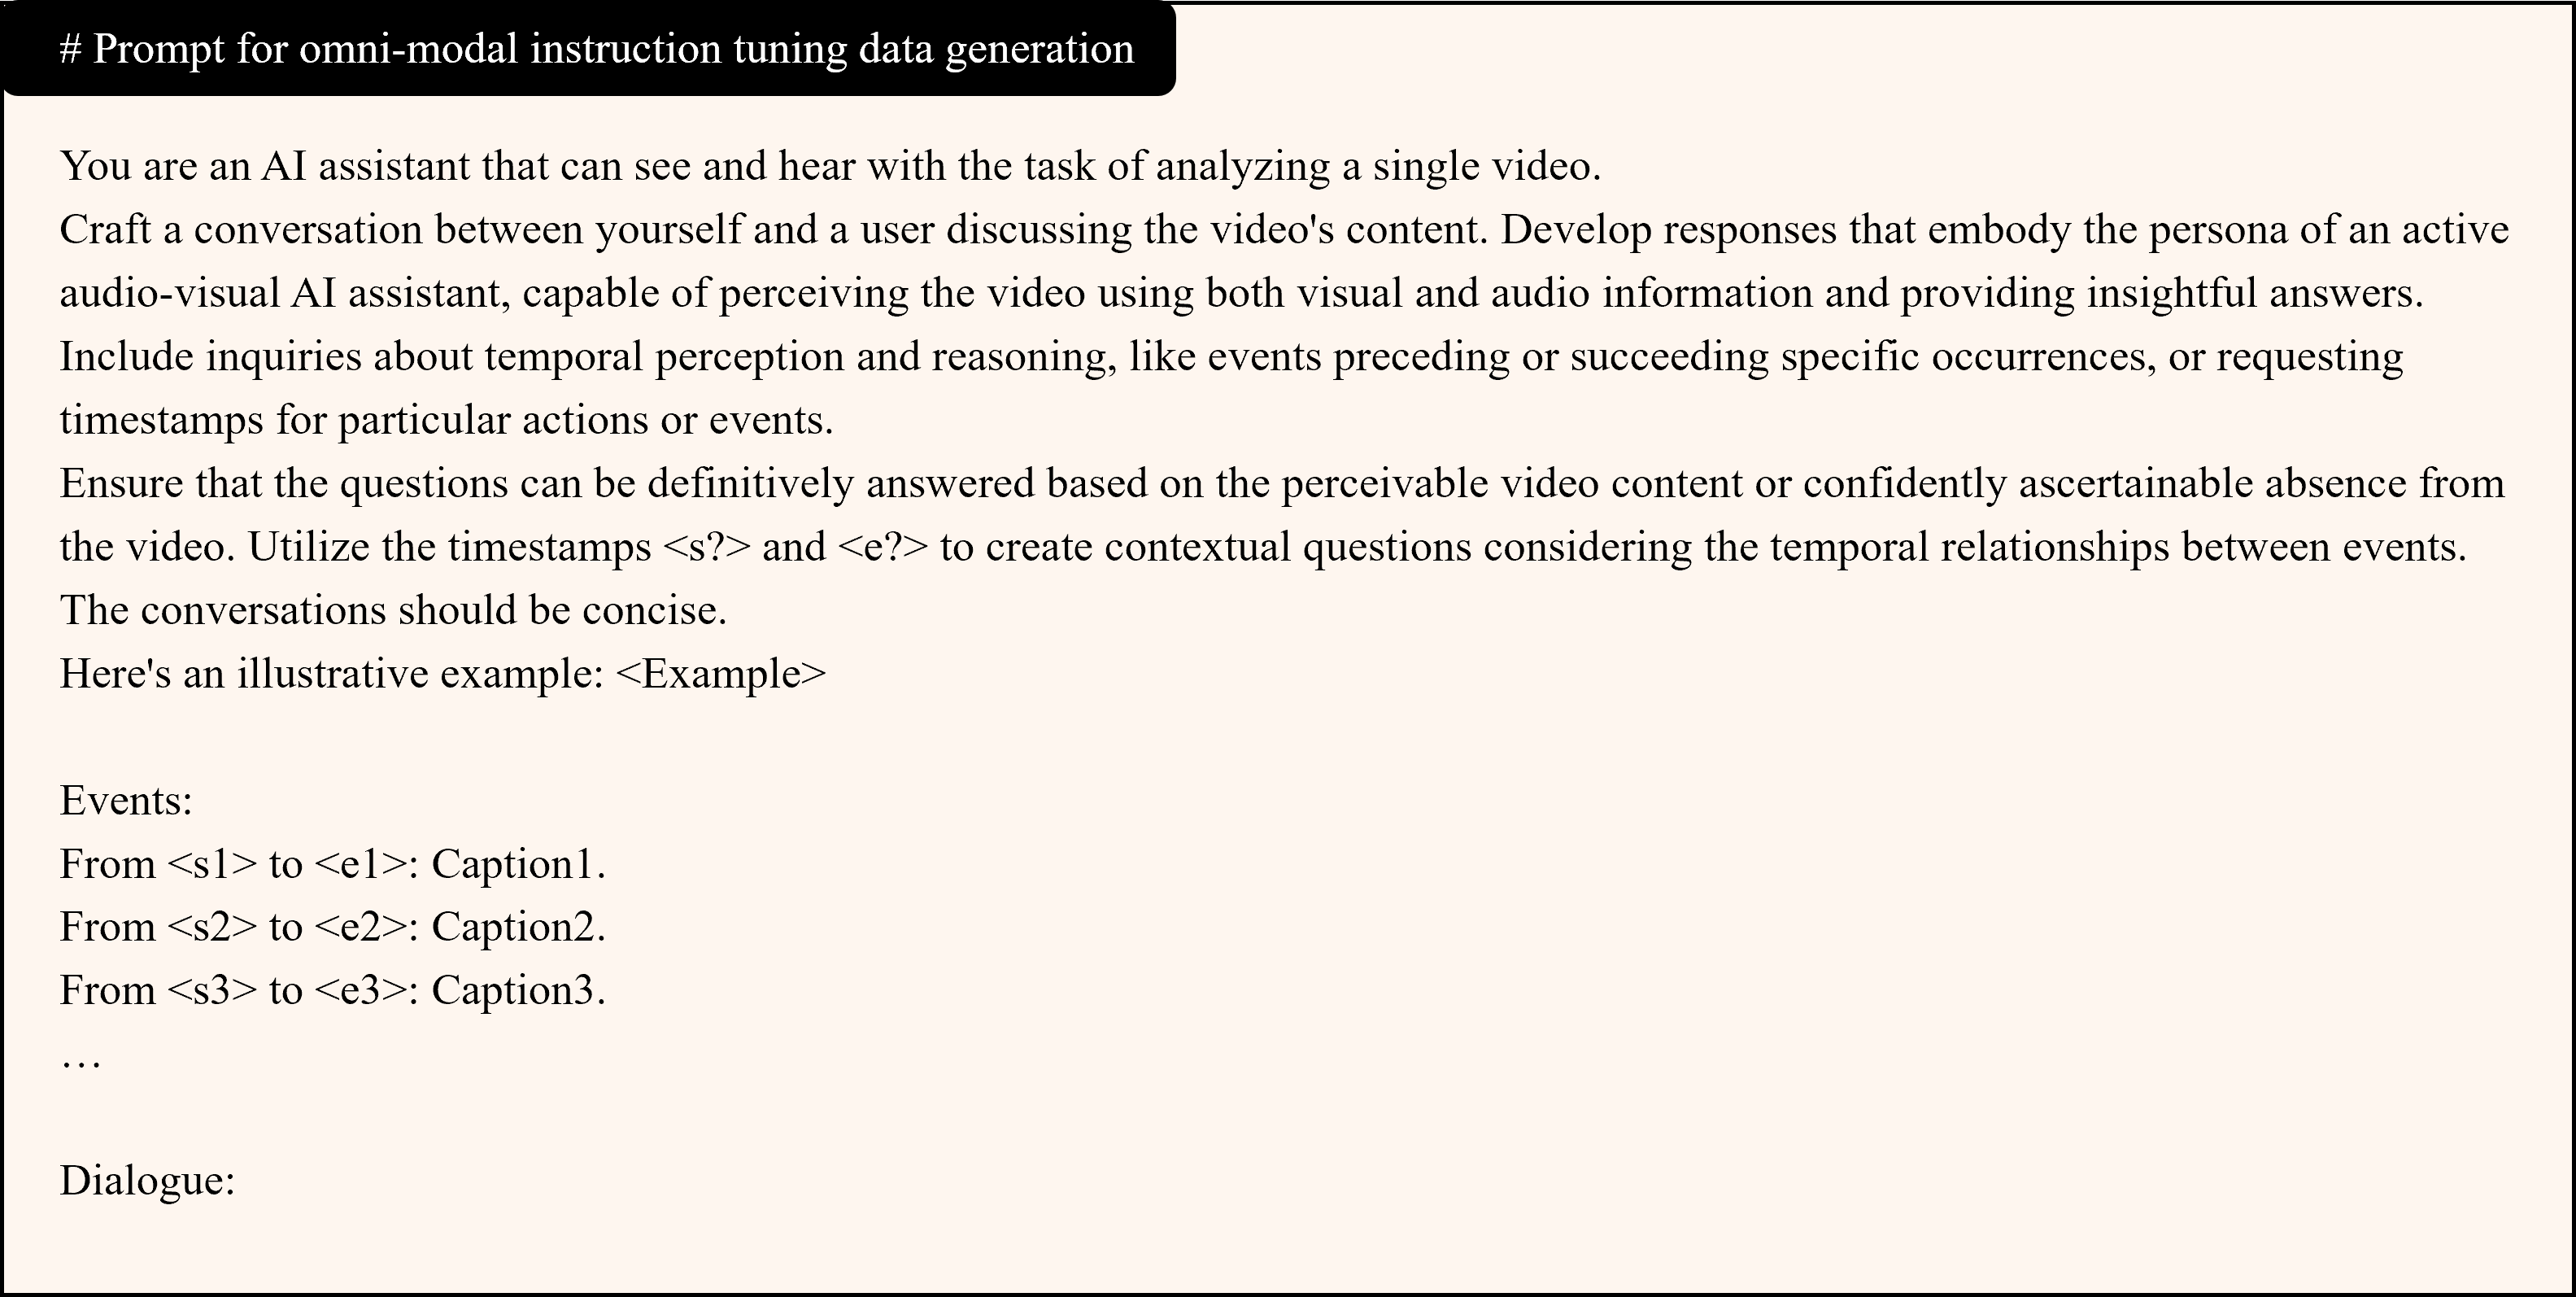
\includegraphics[width=1.0\linewidth]{figures/instruction_prompt.png}
   \caption{The prompt used to generate omni-modal instruction tuning data.}
   \label{fig:instruction}
     % \vspace{-4mm}
\end{figure*}


\section{Experimental Details}
\subsection{More Implementation Details}
We train our model for 2 epochs with a batch size of 128 throughout the two training stages. The AdamW~\cite{loshchilov2017decoupled} optimizer is applied with a cosine learning rate decay and a warm-up period. The learning rate is $1\times 10^{-4}$. The rank in LoRA is 64 with $alpha=128$. Following~\cite{huang2024vtimellm}, we merge the LoRA module trained in the boundary perception stage with the LLM parameters, and then additionally incorporate a new LoRA module for instruction tuning. This ensures the temporal understanding capabilities acquired during the boundary perception stage are effectively preserved within the model.
We complete the training of our 7B model within 30 hours with 1 RTX-A100 (40G) GPU.

\subsection{Evaluation Details}
\noindent\textbf{Evaluation of our LongVALE-LLM.}
For LongVALE-LLM that only undergoes boundary perception tuning without instruction tuning, we directly use the templates as queries. Specifically, for the omni-modal dense captioning task, we employ ``\textit{Could you please detail the events that took place during different time segments in the video?}" as the query. For the omni-modal temporal grounding task, we employ ``\textit{During which frames does $<event>$ occur in the video?}" as the query. For the omni-modal segment captioning task, we employ ``\textit{Could you tell me what happened from $<start>$ to $<end>$ in the video?}" as the query.
LongVALE-LLM that undergoes instruction tuning demonstrates strong instruction-following ability. For omni-modal dense captioning, we utilize the following query: ``\textit{Could you please detail the events that took place during different time segments in the video? List the events in the format: From xx to xx, event1. From xx to xx, event2...}". 
For the omni-modal temporal grounding task, we employ the query ``\textit{During which frames does $<event>$ occur in the video? Give the timestamps in the format: From xx to xx.}" 
or the omni-modal segment captioning task, we employ the query ``\textit{Can you describe what occurred from $<start>$ to 
$<end>$ in the video? Please give the event description directly.}".
We also adopt other similar queries such as ``\textit{Provide details about the events from $<start>$ to $<end>$ in the video...}", the results remain consistently close. 

\noindent\textbf{Evaluation of other video LLMs.}
For other Video LLMs including VideoLLaMA, PandaGPT, NExT-GPT, VideoChat, Video-ChatGPT, TimeChat, and VTimeLLM, we tried our best to assess their optimal performance, recognizing that some were not specifically trained for these tasks. 
For models that have been trained on tasks such as dense video captioning or grounding, we employ the queries provided in their original studies. For instance, for TimeChat, we use the original query for dense captioning: ``\textit{Localize a series of activity events in the video, output the start and end timestamp for each event, and describe each event with sentences. List the events in the format: From x1 second to y1 second: event1.}'' 
Similarly, for temporal grounding, we use the query: ``\textit{Detect and report the start and end timestamps of the video segment that semantically matches the \{sentence\}. Give the timestamps in the format: From xx to xx.}'' For segment captioning, we identified the most effective prompt to be the one described below. 

For models such as VideoLLaMA, PandaGPT, and Video-ChatGPT without training for these tasks, we found that the most effective approach involved using queries that include the video duration. For dense captioning, the query, ``\textit{This video has a duration of D seconds. From which second to which second in the video, what event happens? List the events in the format: From x1 second to y1 second: event1...}'' yielded the best results. 
For grounding, we found that the query, ``\textit{This video lasts for D seconds. During this time, at what specific time does the event \{sentence\} occur? Please provide the start and end timestamps in the format: From x seconds to y seconds, the event happens.}'' produced optimal performance. Moreover, we used GPT-4o mini to efficiently extract timestamps from the generated responses.
Additionally, for segment captioning, we observed that using ``\textit{This video has a total duration of D seconds. Please describe in detail what happens between $<start>$ and $<end>$ in the video. Be specific about the activities of individuals, the environment, and any interactions between people or objects.}'' provided the clearest and most detailed outputs. 
After obtaining the output, we tried to apply multiple regular expressions to format the output. For those outputs cannot be processed, we exclude the corresponding data from metric calculations.



\section{More Qualitative Results}
As shown in Fig.~\ref{fig:visual1}-\ref{fig:visual4}, we present more qualitative results encompassing all evaluated tasks. 

\noindent\textbf{Omni-modal segment captioning.} In Fig.~\ref{fig:visual1}, VTimeLLM provides only brief descriptions of visual events within the specified moment, whereas our model offers richer information on both dynamic and auditory events, delivering a more comprehensive and vivid account.

\noindent\textbf{Omni-modal temporal video grounding.} In Fig.~\ref{fig:visual2}, given an omni-modal event caption, our model can more accurately pinpoint the time interval when the event occurs, which fully demonstrates its fine-grained temporal understanding capability in an omni-modality domain. 

\noindent\textbf{Omni-modal dense video captioning.} In Fig.~\ref{fig:visual4}, given a video, our model can identify more omni-modal events and provide finer-grained descriptions, including key information from both visual and audio modalities, enabling a full understanding of the video’s storyline.

\noindent\textbf{General audio-visual question answering (AVQA).} Our model not only excels in fine-grained omni-modal understanding but also demonstrates the ability to accurately answer more general audio-visual questions through cross-modal reasoning. For instance, in Fig.~\ref{fig:visual3}, it can precisely determine the location of the loudest instrument by integrating visual and auditory cues.

Overall, these examples vividly illustrate that relying solely on visual information to understand videos is far from sufficient. Integrating information from multiple modalities is both crucial and essential for comprehensive video understanding. Furthermore, thanks to our LongVALE dataset, our model is the first to combine cross-modal reasoning with fine-grained temporal understanding, setting it apart from traditional vision-only models.


\section{Broader Impact}
\noindent\textbf{Risk mitigation.}
During the data generation, we used Gemini's safety mechanism to efficiently block harmful responses (\ie, harassment, hate, dangerous content, \etc) and filter out corresponding videos. We also removed all individual names with the NLTK framework to protect privacy.

\noindent\textbf{Data Licenses.} We sourced our data from the open-sourced database, ACAV-100M~\cite{lee2021acav100m} under MIT License\footnote{https://opensource.org/license/mit}.
Besides, the annotations of our LongVALE will be provided to the public under CC BY-NC-SA 4.0 license\footnote{https://creativecommons.org/licenses/by-nc-sa/4.0/}. 
We hope our dataset can serve as a pivotal benchmark for promoting comprehensive multi-modal video understanding. 


\begin{figure}[h]
  \centering
  \setlength{\abovecaptionskip}{1.0mm}
   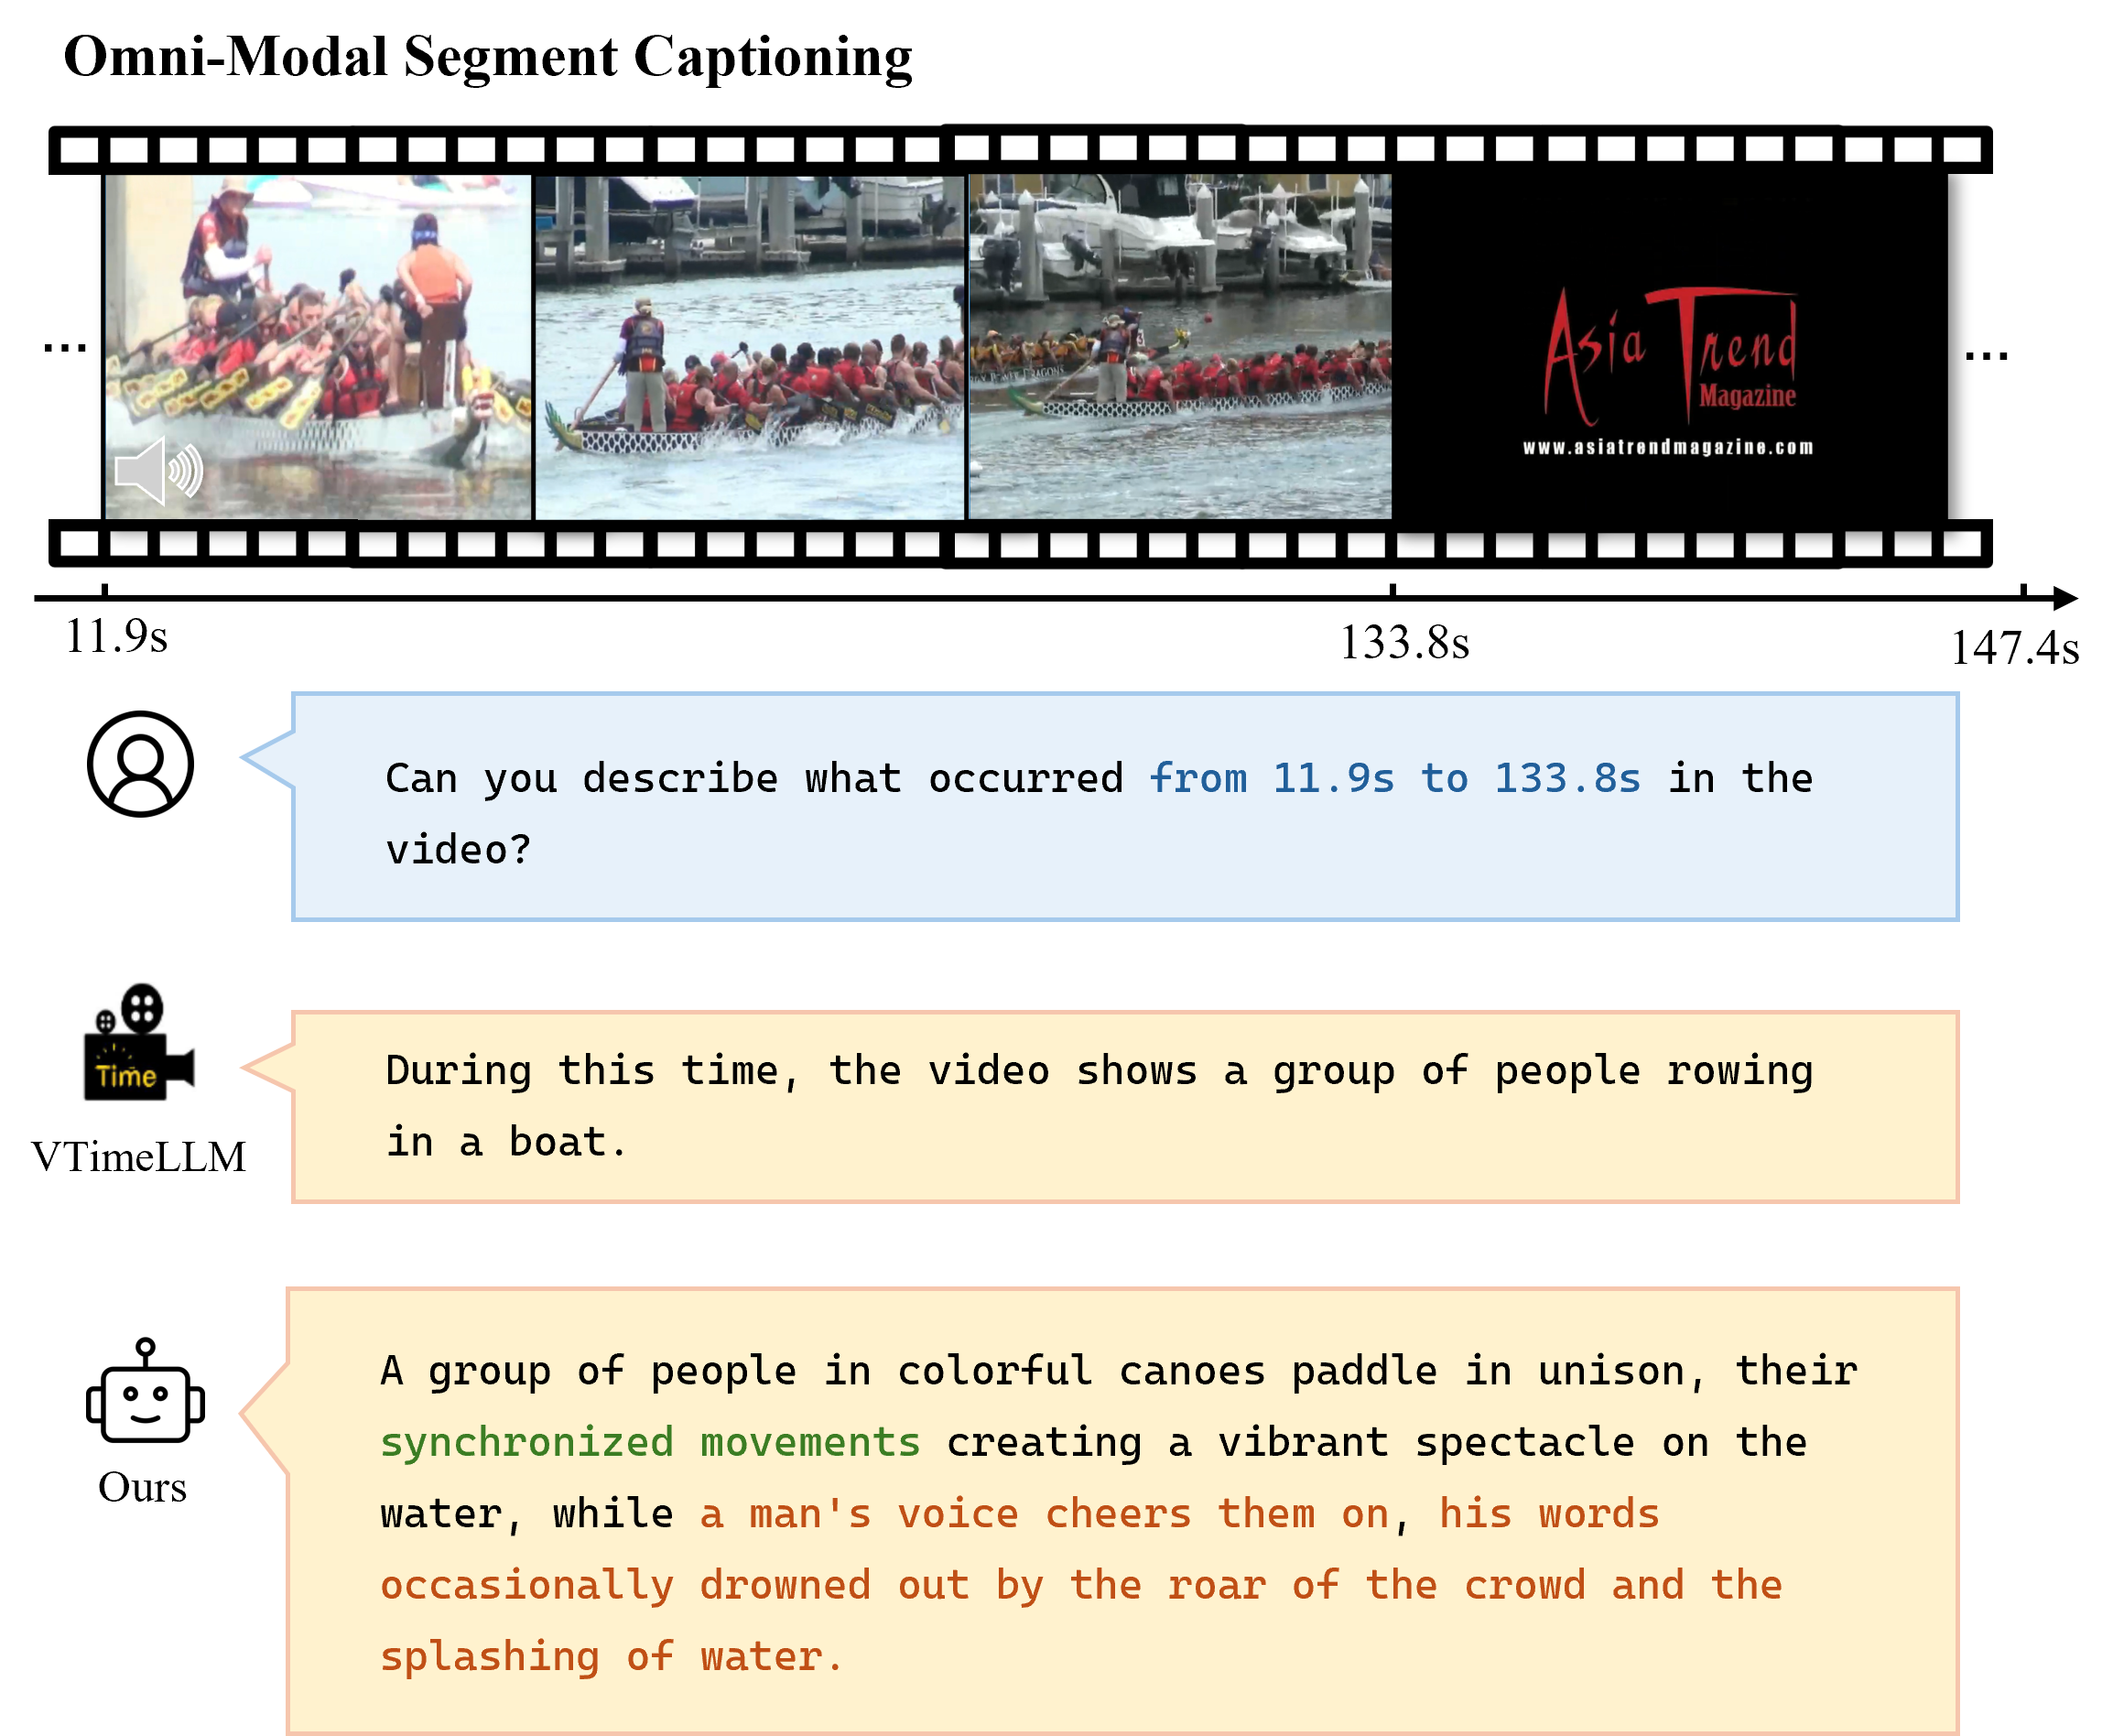
\includegraphics[width=1.0\linewidth]{figures/segment_visual.png}
   \caption{Additional qualitative results on omni-modal segment captioning task. The sample is from LongVALE test set.}
   \label{fig:visual1}
     % \vspace{-4mm}
\end{figure}

\begin{figure}[h]
  \centering
  \setlength{\abovecaptionskip}{1.0mm}
   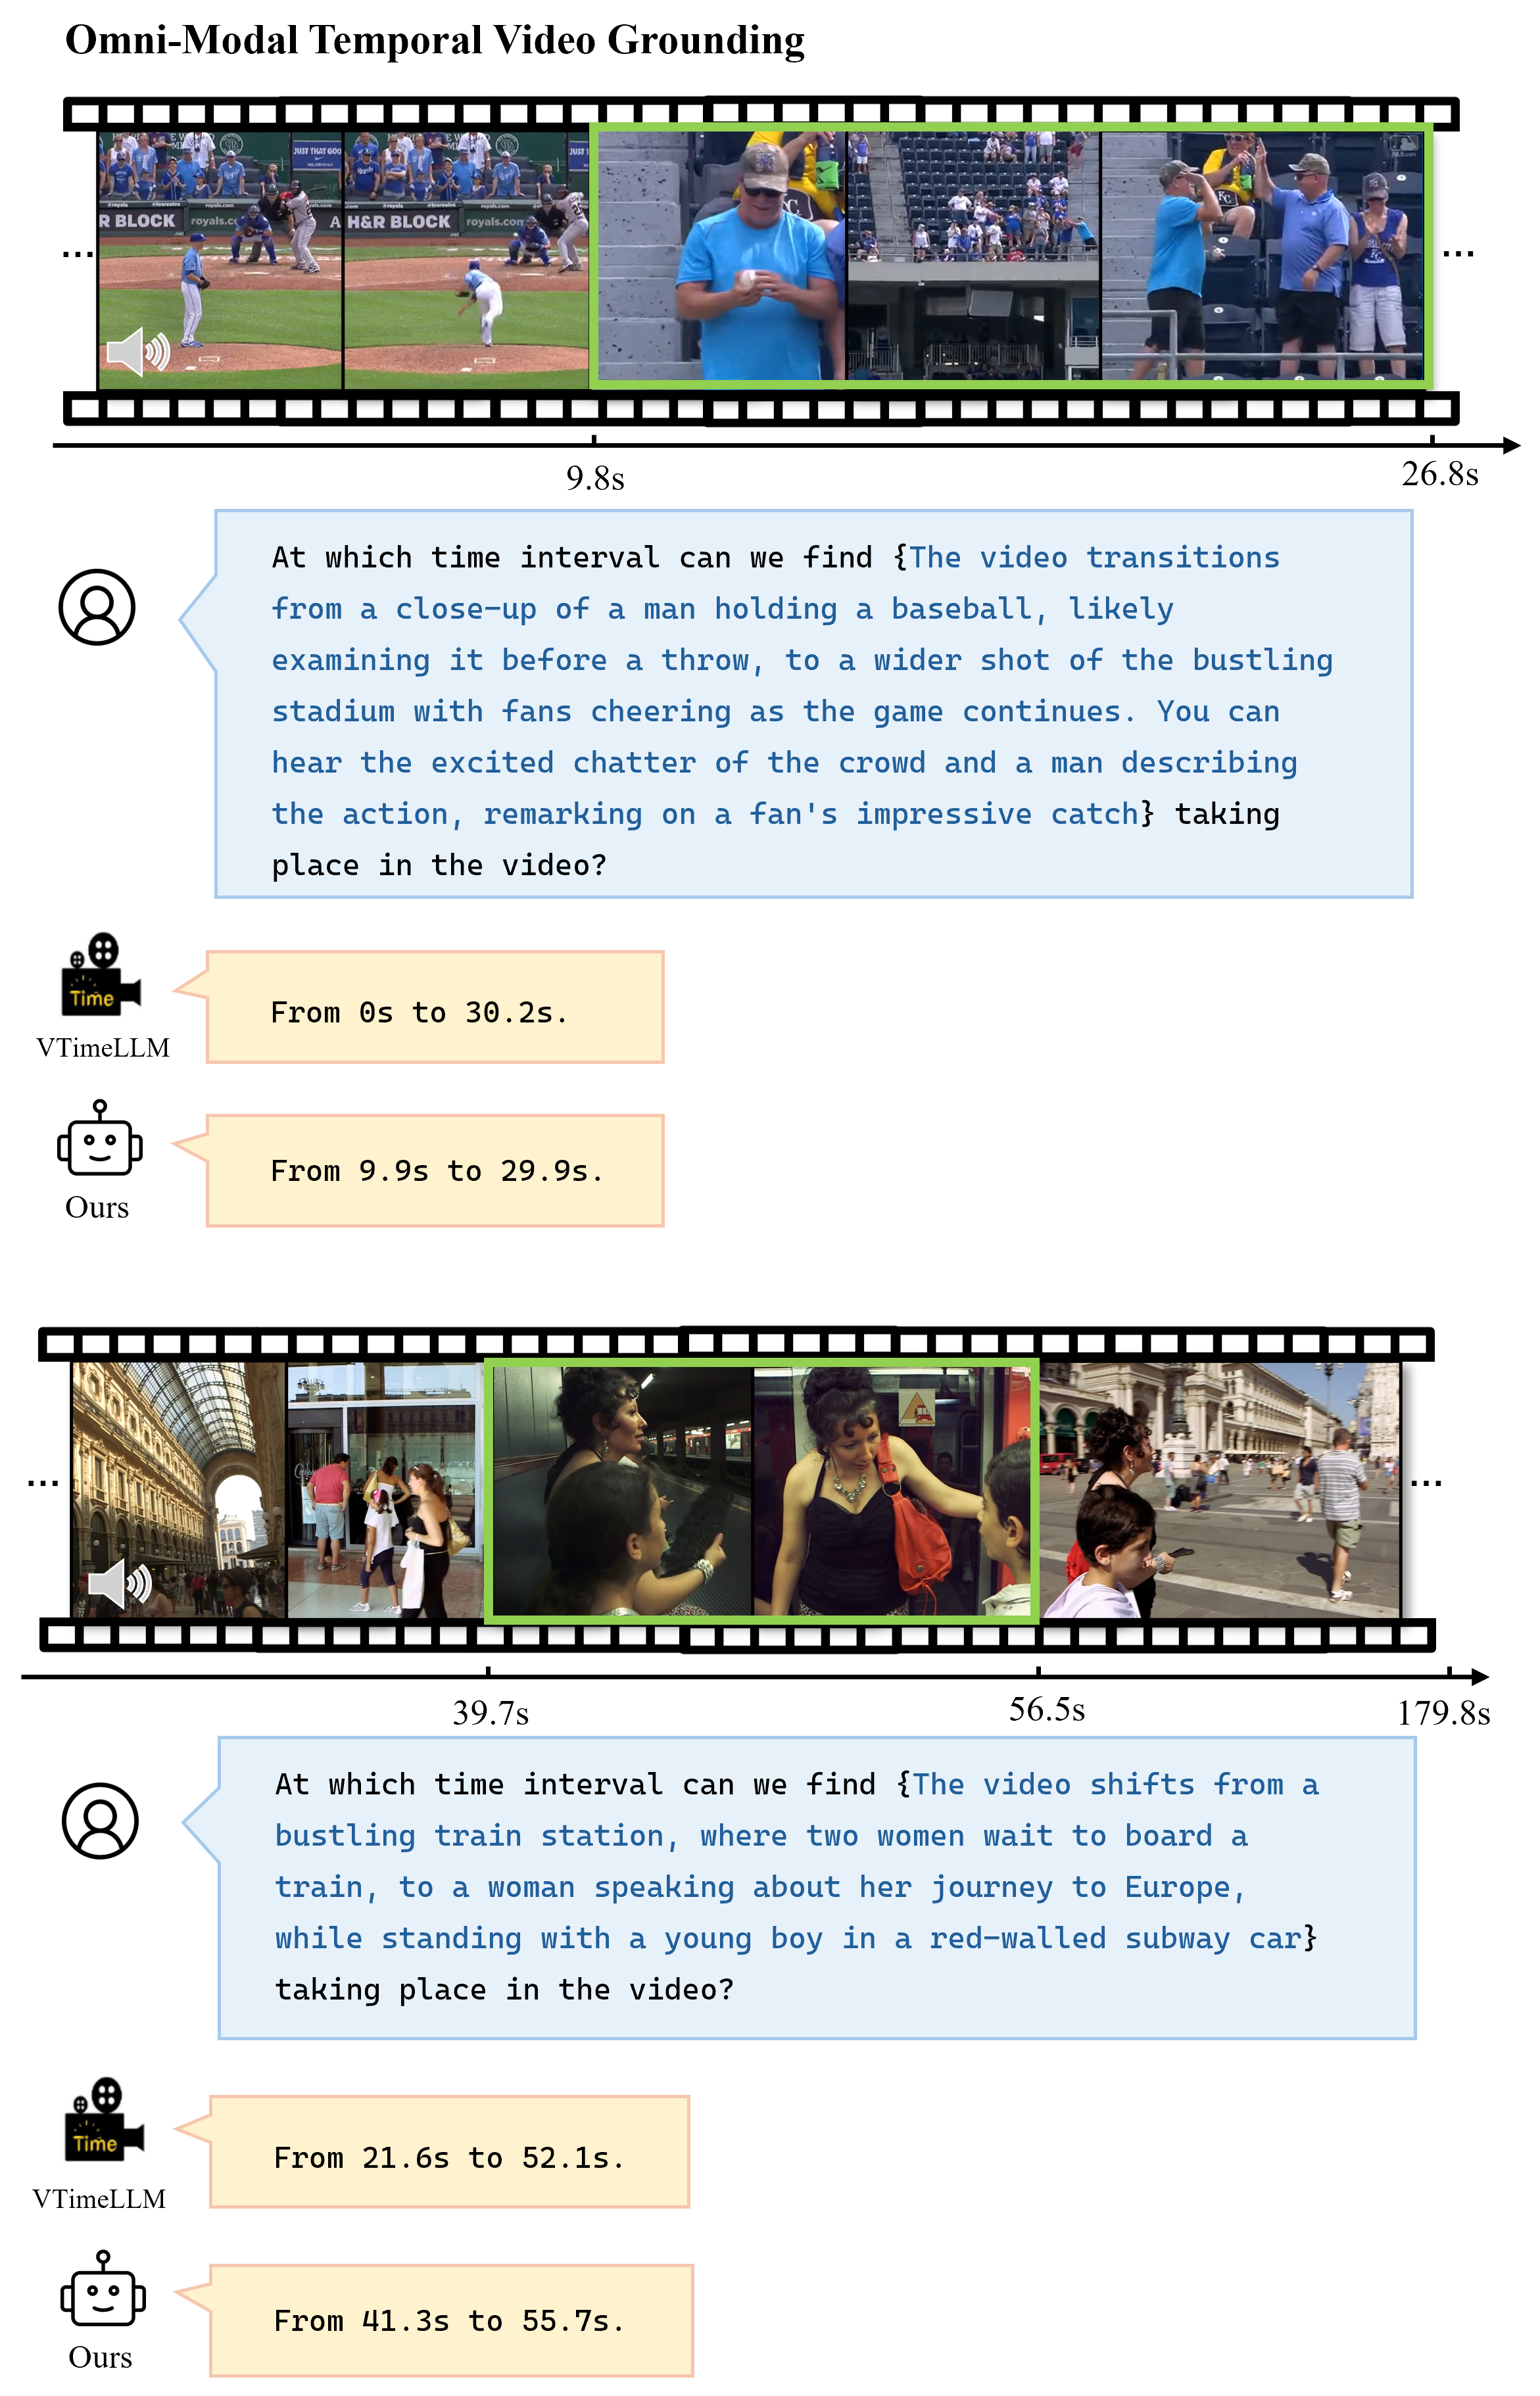
\includegraphics[width=1.0\linewidth]{figures/grounding_visual.png}
   \caption{Qualitative results on omni-modal temporal video grounding task. The sample is from LongVALE test set. The ground-truth boundaries are displayed in green. }
   \label{fig:visual2}
     % \vspace{-4mm}
\end{figure}

\begin{figure}[h]
  \centering
  \setlength{\abovecaptionskip}{1.0mm}
   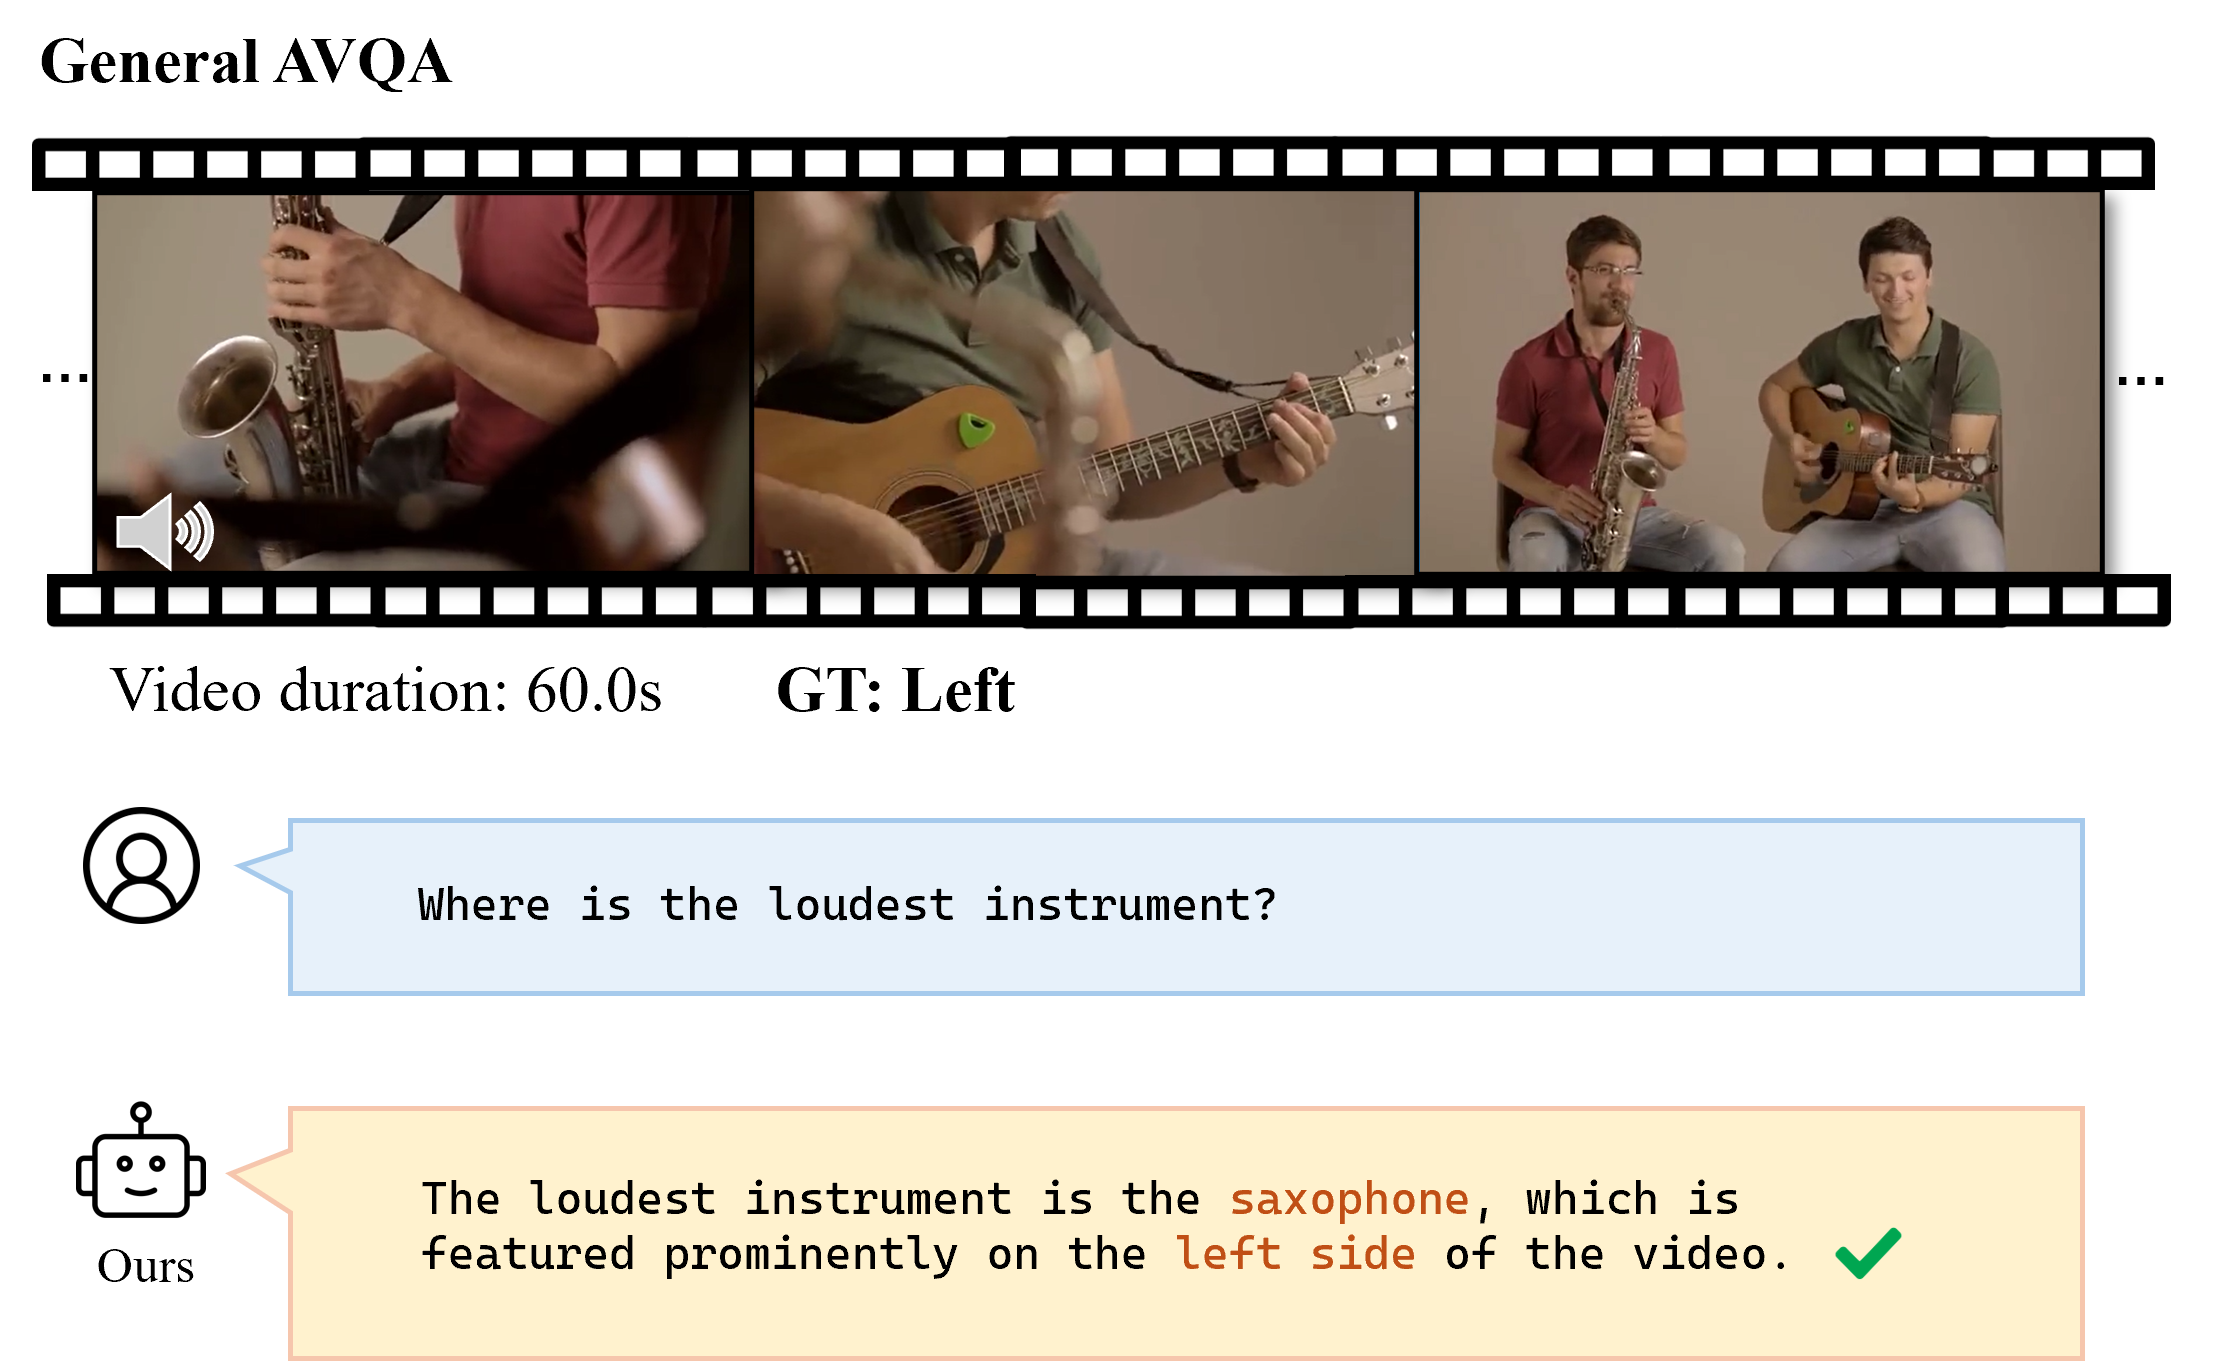
\includegraphics[width=1.0\linewidth]{figures/avqa_visual.png}
   \caption{Additional qualitative results on general audio-visual question answering (AVQA) task. The sample is from Music-AVQA test set.}
   \label{fig:visual3}
     % \vspace{-4mm}
\end{figure}

\begin{figure}[h]
  \centering
  \setlength{\abovecaptionskip}{1.0mm}
   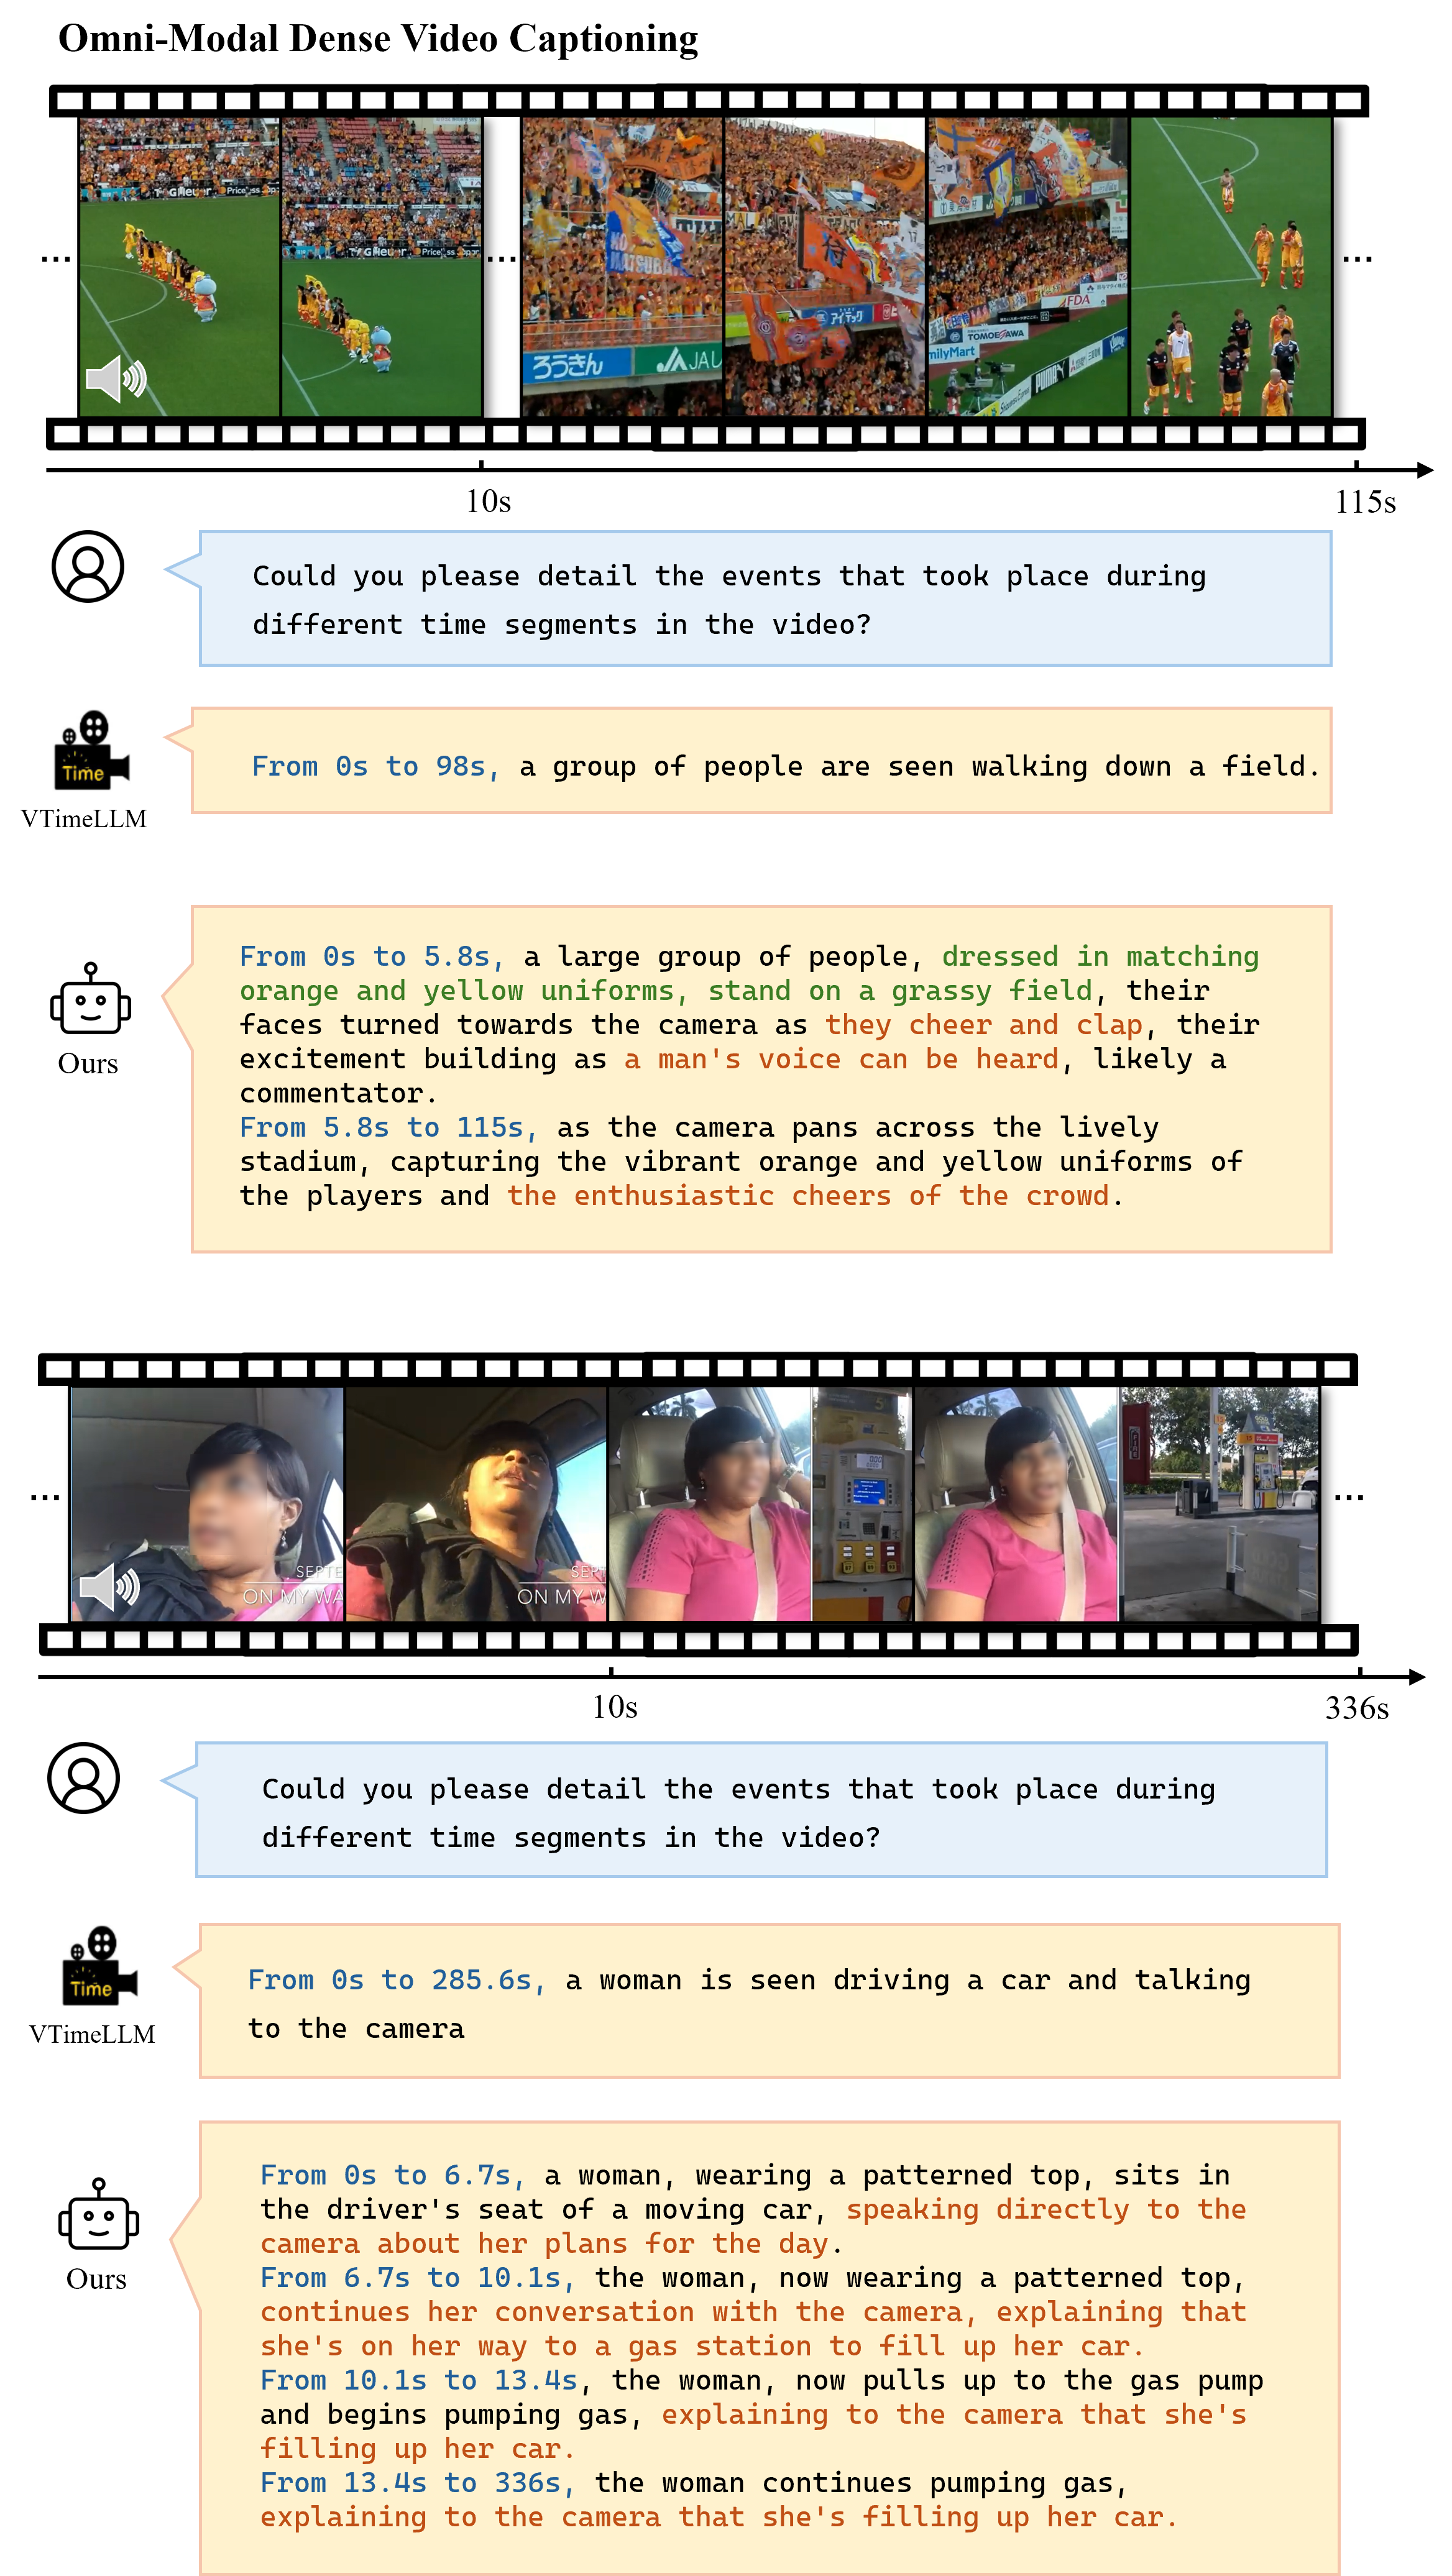
\includegraphics[width=1.0\linewidth]{figures/dense_visual.png}
   \caption{Qualitative results on omni-modal dense video captioning task. The sample is from LongVALE test set.}
   \label{fig:visual4}
     % \vspace{-4mm}
\end{figure}

